\documentclass[11pt,a4paper,twoside]{article}
\usepackage{package/lmuthesis}

\prof{Prof.\ Dr.\ Heinrich Hu{\ss}mann}
\title{Understanding and Predicting\\Web Browsing Behavior}
\author{Changkun Ou}
\email{hi@changkun.us}
\bearbeitungszeitraum{12.8.2018 bis 12.2.2019}
\betreuer{Malin Eiband and Dr. Daniel Buschek}
\aufgabenstellung{
    \begin{description}
        \item[Understanding and Predicting User Browsing Behavior]
 
        \item[Problem Statement] To be added
        % Under standing user behavior helps designer optimize 
        % their product user experiences. Meanwhile, users can benefit more productive 
        % from it. Since user intents are elusive, changeable and sometimes even undetermined, 
        % predict their behavior usually difficult and impoissible. In most cases, a user may 
        % performs a series of wasted actions before reach an intent destination. 
        % Nevertheless, user intents becomes clear step by step after performs a series of 
        % actions in a given context. 
        \item[Scope of the Thesis] To be added
        % To tackle the aforementioned challenges, the objective of this thesis is to develop a system that tracking user actions within a website, 
        % As a first step, literature review ...
        % Based on the literature review, a intent model should be developed ...
        % Then a system should implements the ...
        % Nevertheless, user intents becomes clear step by step after performs a series of actions in a given context. 
        \item[Tasks] (1) Conduct a literature review to identify research questions regarding
        clickstream research that are of interest to researchers and practitioners \\
        (2) Design a machine learning based model in clickstream modeling and 
        creating an appropriate experiment with theoretical support to justify model performance and its interpretability \\
        (3) Develop an web application as a demonstration of the model and evolving it as a generic architecture
        for the proposed model.
        \item[Requirements] Strong skills in mathematical modeling and machine learning approaches, independent scientific work and creative problem solving,
        industrial experience in web development and architecting.
        %asdfasdf
        \item[Keywords] Clickstream, User Browsing Behavior, Machine Learning, Web
    \end{description}
}
\acknoledgement{
    I would like to appreciate Malin Eiband and Dr. Daniel Buschek for many of their great and 
    constructive discussions, suggestion around thesis topic selection, model statements,
    thesis structuring as well as their pacient of given supervision to the thesis. 
    The thesis would not be accomplished without them. Afterward, I am full of gratitude to 
    Prof. Hussmann and Prof. Butz for offering me an unexpected opportunity to study aboard in Germany 
    as well as their kindly helps regarding study and living in my academic period.
    Next, I wish to thank my best friend Yi, schoolfellow Yifei and Xingying, 
    and former colleague Jin for their inspiring discussions surrounding my thesis. 
    Finally, I will forever be beholden to my parents for their continuous supports 
    while my postgraduate study, since they dedicated their live to my better future.
}
\abstract{
Clickstream applications appeared at the end of last century and 
have proliferated at the heart of our Internet world.
Trades, public opinions, and almost every web requests are precisely recorded 
on server-side log files.
The fundamental interaction between a web service client and server stands immutably, 
even though mobile devices have governed our daily life.
In this thesis, we propose a machine learning model that characterizes user browsing behavior 
while including multi-tab branching and backtrack actions in a browser instead of
web request-based clickstreams. We call this model the Action Path model.
To justify our model, we established a lab study and collected individuals' clickstream data, 
which consisted of chronologic URLs and corresponding stay durations for each URL.
We designed nine different contexts given web browsing tasks for three mainstream websites 
based on the theory of information behavior.
Each website has three types of tasks: a goal-oriented task, fuzzy task and 
exploring browsing task. They characterize the corresponding three browsing 
behaviors.
We seek to achieve the following goals by analyzing the subject's trace from our lab study:
1) Understanding: identify if browsing behaviors are distinguishable and 
find common patterns that appear in an action path.
2) Classification: separate and report browsing behaviors on the web, which will help 
users to better understand their status.
3) Prediction: present the future click path in more than one step with the given context of
the browsing history in a session.
Our quantitative analysis indicates that goal-oriented, fuzzy, and exploring
browsing behaviors are classifiable with 100.00\% precision based on the combination of 
chronologic URLs and stay duration. 
The prediction performance of our model indicates higher than 60\% accuracy for 
three to five steps of future clickstream prediction.
Our qualitative analysis of the clickstream indicates five observed patterns, 
including ``ring'',``star'', ``overlap'', ``hesitation'' and ``cluster'' patterns, which 
represent the patterns of an action path. 
To illustrate the application, we also developed a browser plugin that proactively serves users,
and suggests predictions for the possible future user clicks.
Furthermore, we discuss a generalized design of our model and plugin communication protocol. 
This discussion explores the possibility of formalizing the model and protocol as standard 
Web APIs to help designers and developers to improve and monitor the user experience of their products.
To the best of our knowledge, this is the first detailed study regarding web browsing 
behavior modeling based on clickstreams collected from the client side.
}

\begin{document}

\makecover
\makeaufgabenstellung
\makededication
\makeabstract
\maketoc
% \listoffigures
% \listoftables
\cleardoublepage

\section{Introduction}
\label{ch:intro}

\subsection{A Brief History of Clickstream Research}

% 起源

The word ``clickstream'' \cite{friedman1995} was first coined in 1995, a media comments 
article introduced a novel concept of tracing cyberlife of users over the nowadays 
``Internet''. Informally, a ``clickstream'' contains a sequence of hyperlinks clicked by a 
website user over time. At the same year, the most popular server software 
Apache HTTP \cite{apache1995http} proxy on the Web was developed with a feature that 
records access log of entries. Afterwards, people realized the potential danger and value 
of tracing cyberspace, which a large discussion of clickstream influences, such as 
frequency based mining of clickstream \cite{brodwin1995}, privacy concerns 
\cite{reidenberg1996governing}, and database schema of session based time series data 
\cite{courtheoux2000database}.

% 搜集 clickstream 带来的推动

Privacy discussion concludes collecting traces over net clearly offence the rights of users,
the practice violates the openness and transparency of a service to a user.
Serious criticism arise the tracing becomes a loss of democratic governance \cite{gindin1997lost}.

Technologies is not guilty. After years of discussion, positive opinion proposes the rules 
\cite{reidenberg1996governing} and regulations \cite{skok1999establishing} in cyberspace,
means of protecting information privacy in cyberspace transactions \cite{kang1997information},
and approaches to resolve conflicting international data privacy \cite{reidenberg1999resolving}.

Meanwhile, bussiness man agilely responses to the concept and immediately initate 
commercial tracking of their customer to improving marketing affects \cite{novick1995}, 
customer service and precise advertisment\cite{reagle1999platform, bucklin2000sticky}, 
even measuring product success \cite{schonberg2000measuring}.

At the turn of this century, common reviews start accept the technology of clickstream,
clickstream data has confirmed by industrial practice, which opens a new era in 
customer service \cite{walsh2000internet}, most of website users start accept their click path data 
be aggregate analysed on the server side \cite{carr2000hypermediation}.

Clickstream data grows fast and becomes plentiful, researchers start convey the original concept of clickstream,
tracking customer selections, into various applications, such as usability testing \cite{Waterson:2002:LOW:506443.506602},
understanding social network sentiment \cite{Schneider:2009:UOS:1644893.1644899}, and developed visualizing
technique to better interpret clickstream data \cite{Waterson:2002:DTU:1556262.1556276}.

Analysis, reports and characterizing of clickstream gains its popularity, Mobasher et al. \cite{Mobasher:2001:EPB:502932.502935}
suggests personalize user based on association rule from their web usage data. Chatterjee et al. \cite{chatterjee2003modeling} 
first proposed E-commerce websites should use clickstream to tracking customer navigation pattern instead of essential choice, 
associating and binding products for observing responses of a customer.

With the arise of characterizing and behavior understanding on clickstream data, more 
and more research proposes methods for the understanding of given server clickstream data.
Padmanabhan et al. \cite{Padmanabhan:2001:PID:502512.502535}
proposed an algorithm to address personalization from incomplete clickstream data, which implies
a security problem potential information leak from clickstream data. 
Moreover, affected by search engine indexing, Lourenco at al. \cite{Lourenco:2006:CWC:1145581.1145634} recommends an approach for
the detection and containment of web crawler based on server side recorded visiting log file.

After a short review of clickstream history, almost all research putforwards their 
methodology based on server recorded clickstream data.
Note that a daily user is always allowed accesses parallel pages and windows simultaneously,
even allow switching across multiple websites for a browsing purpose.
An obvious missing aspect of those papers is the server recorded data tend to incomplete for 
characterizing a visited user, and the log data can only applied on a specific website. 
As an observation, our research no longer surves server side clickstream, 
but focus and contributes to a client side collected clickstream data 
for a real visiting session of a user in a browser.

\subsection{This Thesis}

% 大体上介绍本论文想要研究 clickstream 的内容,
% 这包括如何开展 clickstream 数据的搜集工作,搜集任务是什么,主要使用的方法,
% 以及得出的结论。根据这些结论,文章提出了一个客户端的插件,
% 能够在现代浏览器上支持这样的预测,
% 同时还进一步探讨了此项功能作为浏览器内建功能甚至浏览器 API 的可能性。

% 本文将视线移出服务端点击流数据,将焦点转移到客户端点击流数据,尝试对客户端独立用户的点击流进行解释。
% 本thesis 由以下几个部分组成。

The main part of the thesis is structured in different chapters, and answers the following
three research question groups:

\begin{enumerate}
    \item \textbf{Understanding}: Why collecting clickstream on client-side differs 
        from server-side collecting?
        What are the most significant, identifiable user behaviors and activity patterns 
        can be observed or algorithmically detected in the context of web browsing that 
        indicates information needs,
        and in which form of quantitative data can characterize a definitive boundary to 
        distinguish browsing behaviors of a user?
    \item \textbf{Classification}: How accurate or how affirmative we can model or identify 
        the proposed browsing behaviors progressively that makes an intelligent system 
        serves proactively?
    \item \textbf{Prediction}: How much future movements of a user can be accurately inferred 
        from the context of web browsing, and how much context is required for the prediction?

\end{enumerate}

% 第二章讨论了目前已有的客户端点击流研究。
Chapter \ref{ch:relate} discusses the exitsting user behavior research based on clickstream data firstly. 
Then discussed the evolution of theory regarding information seeking behavior as our experiment foundation.
In addition, we summaried the reason of recent raise of neural approach in different scientific 
area and the state-of-the-art approaches for generic sequence learning, whose proposed in neural network research.
% 第三章介绍了我们的数据类型、模型的设计。
Chapter \ref{ch:model} defined the completion effeciency of a clickstream first, then we
formalizes our proposed sequence to sequence encoder/decoder model for client-side
clickstream as well as the training techniques for the proposed model.
% 第四章详细描述了实验的设计,介绍了每个所设计任务的原因和考虑,讨论了每个所设计的任务中潜在的数据的搜集和分析工作。
In subsequent chapter, Chapter \ref{ch:exp}, we present our experiment for a lab study,
and construe the design reason of context given web browsing tasks for our subjects based on information behavior theory.
% 第五章分析了第四章描述中搜集到的数据,基于 SVM、t-SNE 分析了除了点击流之外的几个特征,定量分析,得出了结论。。。。
% 然后基于第三章中提出的模型,分析了。。。。的结果,得出了。。。的结论。
Afterwards, in Chapter \ref{ch:eval}, based on SVM, t-SNE and our proposed model, 
we conducte a quantitative analysis with described data from our lab study, 
the evaluation shows a very promising results.
% 最后对用户在任务下的点击流进行了可视化,定性分析,进一步讨论了用户的行为,从而进一步验证了我们的结论。。。
Moreover, we visualize the clickstream through directed graph, by combining our traning model outputs,
we also performs a qualitative analysis to all clickstreams, and the analysis gives evidences that further 
verified the correctness of our model.
% 第六章首先介绍了浏览器插件的工作原理,讨论了我们插件的工作架构。介绍了插件的客户端和服务端的实现方案。
In Chapter \ref{ch:app}, as a consequence of our analysis, we developed a browser plugin 
for Google Chrome as a possible application to our model. The plugin can fairly predict 
the next possible visiting pages of a user. In addition, we generalize the design of
our plugin architecture between client and server,
and then discusse the possibilities of being a standard web API to web developers.

% 第七章对整个 thesis 进行了总结,讨论了本文工作中存在的不足以及未来可改进的方向。
In the last two chapters, we discusse the limitations of this work, summarize the findings of our thesis, 
as well as the possible future improvements and directions of the thesis in the final chapter.
\cleardoublepage
\section{Related Works}
\label{ch:relate}
\epigraph{If I have seen further it is by standing on the shoulders of Giants.}{Isaac Newton}

% - 讨论 client-side 的 clickstream 为什么值得研究,比较服务端搜集的 clickstream 产生的明显变化是什么。
% - 讨论现有的 client-side clickstream 研究分别是针对什么方向的,他们的结论主要是什么,都有什么样的改进空间。
% - 以前的 clickstream 只有类别级的分配模型,通过人工设计某个特定网站的马尔科夫模型来学习用户在不同类别之间的跳转概率。但当变为客户端后,数据变得更加充分,用户在一段时间内可能不局限于某个特定的网站,同时可能被其他网站干扰。

In this chapter, we discuss the former research that releats to our work, including
the existing approaches to clickstream behavior modeling, the evolution of information 
behavior theory regarding how it adapts to our digital world, as well as the 
most related recent advances regarding sequence learning.

\subsection{Clickstream Behavior Modeling}

Clickstream behavior research can be traced back to the year when the word ``clickstream''
was invented. Eearly clickstream behavior research studied the navigational behavior
of user \cite{mandese1995clickstreams, brodwin1995} and 
they binary classified clickstream based on the degree of linearity.

Mobasher et al. discovered the effective and scalable techniques \cite{Mobasher:2001:EPB:502932.502935} for Web personalization
by using association rules and built a recommondation system. Goldfrab invistigates \cite{goldfarb2002analyzing} 
the website choice behavior based on clickstream data and suggests that clickstream simulate company strategy changes.
Afterwards, 
Chatterjee et al. \cite{chatterjee2003modeling} first conduct 
the previous research regarding clickstream to an actual commercial website.
They found that clickstream represents an implication that dynamic advertising
based on customer clickstream history influence the future clickstream of the customer
and increase the interaction with the dynamic advertisement.
More techniquely, Ting et al. uses common sequences to find unexpected browsing behavior \cite{Ting:2005:UMF:1092358.1092469},
and then use their findings to improve website design. 

The most recent research evolved the approach of clickstream modeling,
Wang et al.\cite{Wang:2016:UCC:2858036.2858107} proposed a unsupervised appraoch to model clickstream without labeling.
Chi et al. proposed an analysis framework \cite{chi2017towards} for the general understanding of online information behavior
in a specific page. However, their framework only fits for server side collected clickstream other than a real user clickstream.
Then, Wang et al. \cite{Wang:2017:CUB:3127338.3068332} improved their unsupervised appraoch,
and summarized more approaches for clickstream behavior modeling that identifies span ad abuse
for a specific website. Park et al. models and detects a behavior change among student while learning 
based on Poisson process \cite{Park:2017:DCS:3027385.3027430} to
help improve online learning experience. Amo et al. \cite{amo2018learning} further visualizes search-stream
behavior based on student clickstream on a class, and Shimada et al. proves \cite{Shimada:2018:OCD:3170358.3170412}
online change detection while monitoring on student behavior is possible based on a sliding window.

Zaloudek gives an review on the comparasion \cite{mastersthesis} traditional method to model clickstream data,
then proposed a principle component analysis based method for a semi-supervised learning
of clickstream data, however their approach does not work well on clustering task, and 
the best performance is obtained by traditional multilayer perceptron algorithm.
Chandramohan and Ravindran then further investigate the neural approach on clicksteam mining \cite{N:2018:NAB:3152494.3152505},
they verified that complexy LSTM with Attention mechanism is able to capture whether a user
is intent to buy a product or not based on server side collected clickstream.
Surprisingly, Gundala and Spezzano \cite{Gundala:2018:RDH:3184558.3191644} simply use a Lasso
regression based on sofisticated feature engineering 
archived AOC score 0.769 for reader demand hyperlink prediction on Wikipedia clickstream dataset.

Kammenhuber et al. is the first study regarding client side clickstream \cite{Kammenhuber:2006:WSC:1177080.1177110}.
They proposed a finite-state Markov model that models user's search behavior on a level of
topic categories. Unfortunately their dataset are collected from network package traffic,
and did not consider the time a user spend in each page.


% 关于 assistent 的研究
% @article{lieberman1995letizia,
%   title={Letizia: An agent that assists web browsing},
%   author={Lieberman, Henry and others},
%   journal={IJCAI (1)},
%   volume={1995},
%   pages={924--929},
%   year={1995}
% }

\begin{figure}[H]
    \centering
    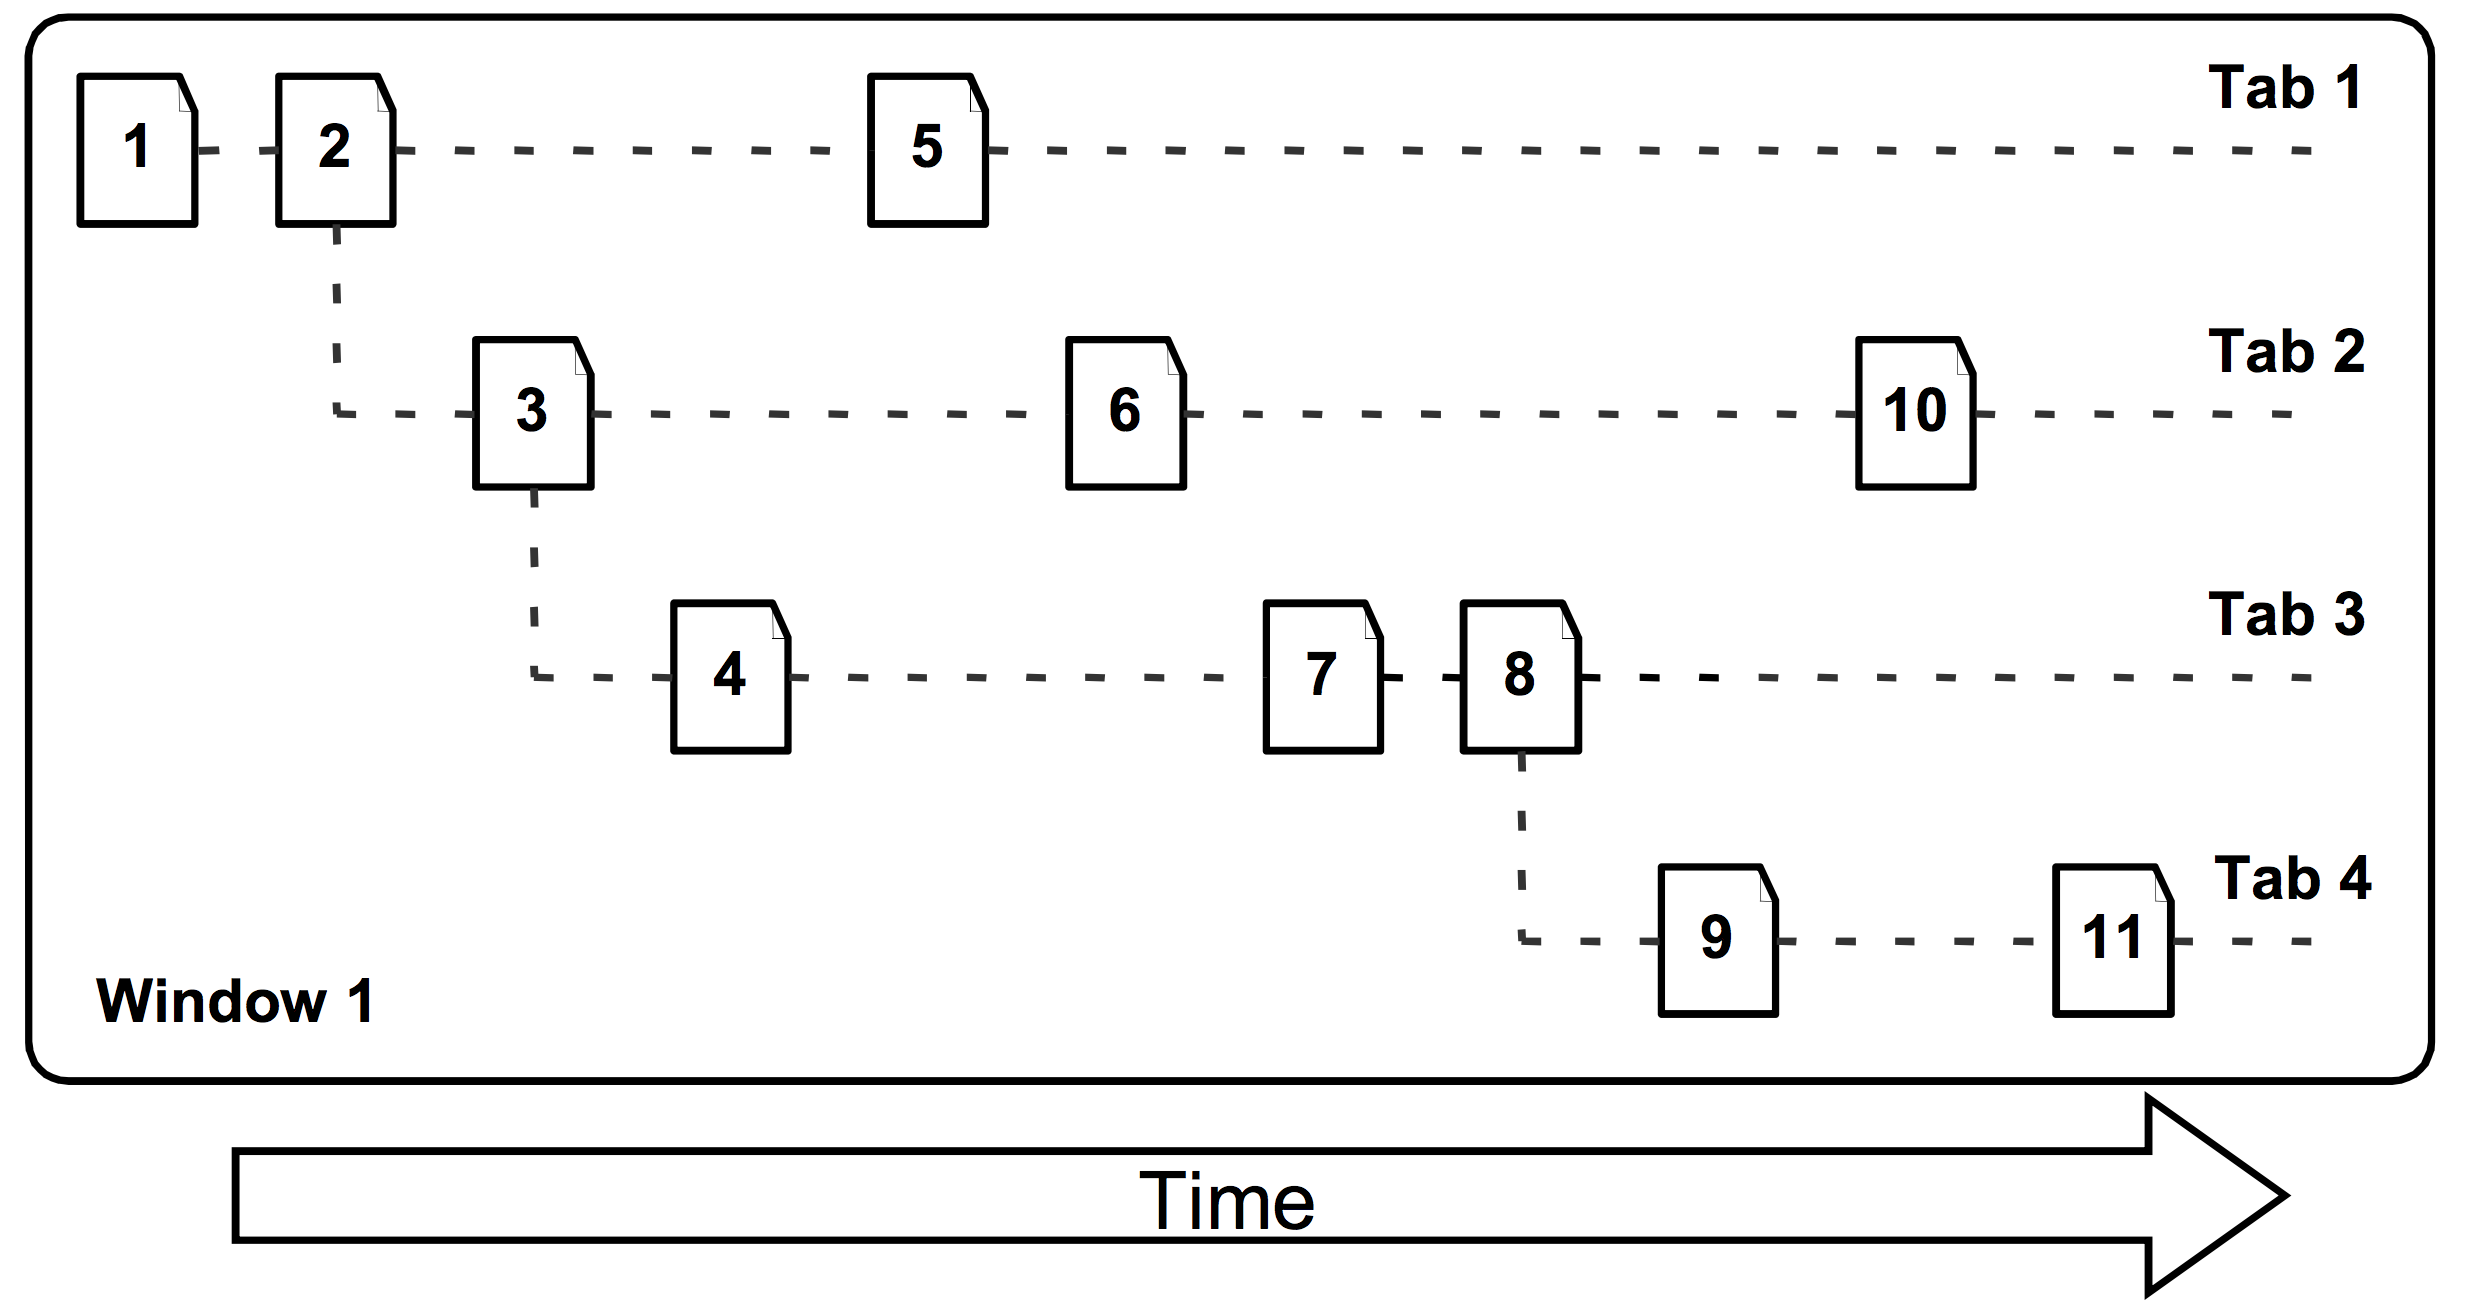
\includegraphics[width=0.55\textwidth]{figures/branching-and-backtracking}
    \caption{Parallel browsing behavior: branching phenomenon \cite{huang2010parallel}}
    \label{fig:backtrace}
\end{figure}

Liu et al. \cite{liu2010understanding} studied a specific user behavior on dwell time on web pages, and concluded that
Weibull distribution is the most appropriate distribution to characterize this behavior. 
Huang et al. \cite{huang2010parallel, huang2012no} further 
noticed the behavior of branching parallel browssing and backtracking browsing
behavior on modern browsers, as shown in Figure \ref{fig:backtrace}, 
and presented an frequent analysis for the distribution of these two behavior individually.

Unfortunately, as we discussed above, the existed research regarding clickstream 
behavior modeling are either server-side modeling for an individual client or 
individually modelized for client-side behaviors with limited information of clickstream,
which does not stands for a real user behavior. 
Besides, the existed approaches are based on self-constructed features, 
the property of Markov memoryless and etc. Though the most recent
approach use neural networks, their findings only applies to specific context.

From the point of view of user behavior, they 
neither unambiguously justifies the foundation of their model, 
nor providing a significative performance of their model.

We, in this thesis, serialize the client side chronologic URL sequences with combines all 
these individually studied phenomena including the branching and backtracking browser 
feature. With this chronologic URLs, we seek to model and understand the essential user 
behaviors patterns while browsing on the Web.

\subsection{Theory of Information Behavior on the Web}
\label{sec:info-seek}

The thesis relates to information behavior theory since it supports the foundation of our
user study. This subsection discusses how the theory was concluded and 
the principles of the theory that sustain our thesis.

Information behavior research encompasses intentional information seeking and 
unintentional information encounters, and the roots to information behavior 
theory relates to information needs and uses \cite{doi:10.1002/aris.2009.1440430114} 
that arose in the 1960s.

However, the concept of information seeking behavior, was coined in late 1981 
by Thomas Wilson \cite{wilson1981user}, and he tries to formalize the process or 
activities of a conscious effort while information needs 
and uses. Figure \ref{fig:wilson-info-seek} illustrate the model of information behavior 
was proposed.

\begin{figure}[H]
    \centering
    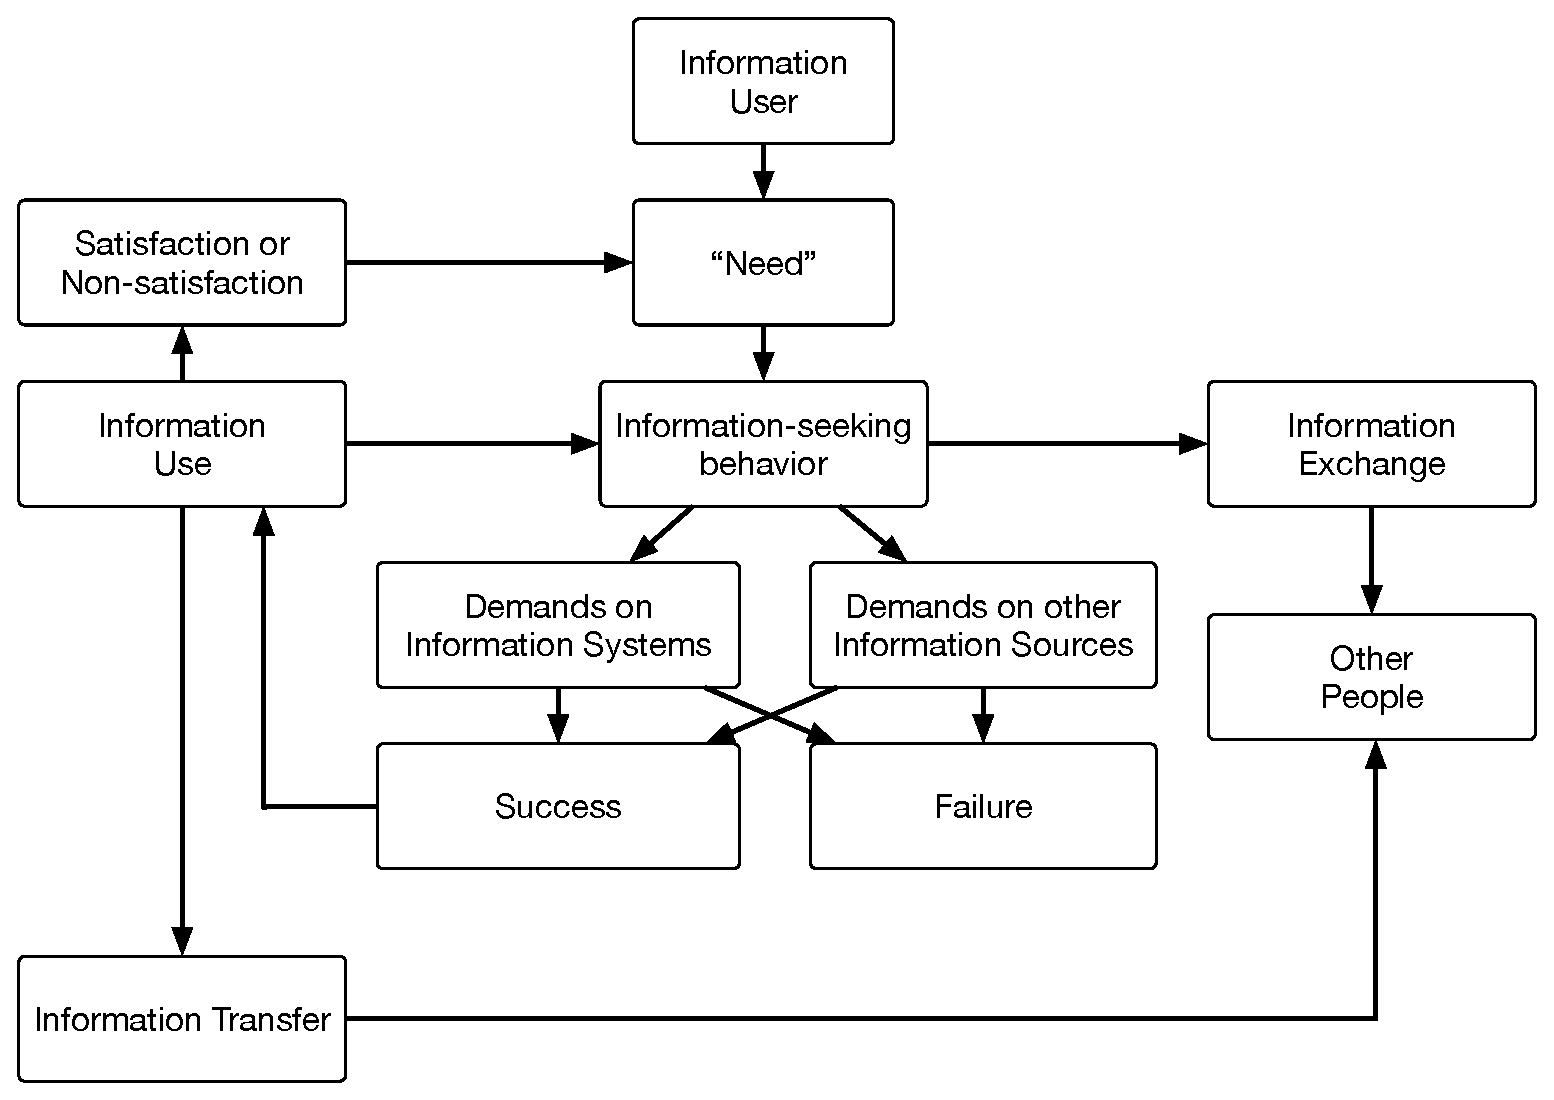
\includegraphics[width=0.7\textwidth]{figures/wilson-info-behavior}
    \caption{Wilson's information seeking behavior model \cite{wilson1981user}}
    \label{fig:wilson-info-seek}
\end{figure}

Wilson's model has been envolved many years since its origin, and it was revised 
and adapted to our digital world since the digital systems learns user preferences and 
changes \cite{giannini1998receiving} the way we receiving information.

David Ellis described a detailed group of activities for information seeking behavior \cite{ellis1989behavioural},
and then applied in physical and social science \cite{ellis1993comparison} and industrial
environment \cite{ellis1997modelling}.
In addition, his analysis was
based on grounded theory approach \cite{aceto1994grounded} and semi-structured interviews. 

Afterwards, Choo et al. adapts Ellis' Model and discussed \cite{choo1999information}
the information seeking behavior on the web through different activities rather 
than a single process, the applied activities are:
starting, chaining, browsing, differentiating, monitoring, and extracting.

``\emph{Starting}'' on the web indicates that a user identifies websites or pages
that containing the information of interests.
``\emph{Chaining}'' indicates that a user follows on starting page to other related pages.
``\emph{Browsing}'' then represents the activity that a user only skimming on the web
and quickly viewing the top-level informations. The ``\emph{differentiating}'' 
describes that a user on the web is selecting useful pages and choosing differentiated.
``\emph{Monitoring}'' activity is used for receiving updates on the sites, or revisit
the previously visited pages. Finally ``\emph{extracting}'' is the activity that a user
systematically extracts informations from a interested page or website.

By applying these activities, Choo et al concludes general user behaviors on the web are
undirected viewing, conditioned viewing, informal search and formal search.
Johnson further describes \cite{johnson2017patterns} seven more detailed behaviors 
patterns on the web, but did not given a working study that verify or prove their formation.

Although Wilson's model and Ellis' model are revised in recent works, however these improvements
are more generic and too complexy for describing user information behavior on the web.
Therefore, in this thesis, we only uses the an antecessor of Wilson's framework \cite{wilson1997information} and 
Ellis' model \cite{ellis1997modelling} to formalize and justify our lab study experiment later in Chapter \ref{ch:exp}, 
as a fundation of our work.

% \subsection{Theory of Sequence to Sequence Learning}

\cleardoublepage
\section{Action Path Models}
\label{ch:model}

\epigraph{It is impossible to separate a cube into two cubes, or a fourth power into 
two fourth powers, or in general, any power higher than the second, into two like powers. 
I have discovered a truly marvelous proof of this, which this margin is too narrow 
to contain.}{Pierre de Fermat}

In this chapter, we formalize few concepts and metrics in clickstream data,
and then describe a proposed clickstream model named \emph{Action Path model} 
based on a recurrent neural network that models a client-side web browsing behavior. 
An \emph{action path} is different than the original clickstream concept since 
a user may \emph{switch browser tabs} for parallel viewing \cite{huang2010parallel} 
or uses \emph{back button} 
for backtracking viewing \cite{huang2012no} as we discussed in Chapter \ref{ch:relate}, 
namely, a user performes a visit action.
A server-side collected clickstream does not contain such detailed level of user clickstream.
The term \emph{action path} is a generalized concept of clickstream, 
which replaces individual URLs to chronological ordered user actions 
(with back button and browser tab switch effects) in a browser.
Figure \ref{fig:clickstream} illustrates a simplified version of an action path 
that compares vanilla clickstream.

\begin{figure}[H]
    \centering
    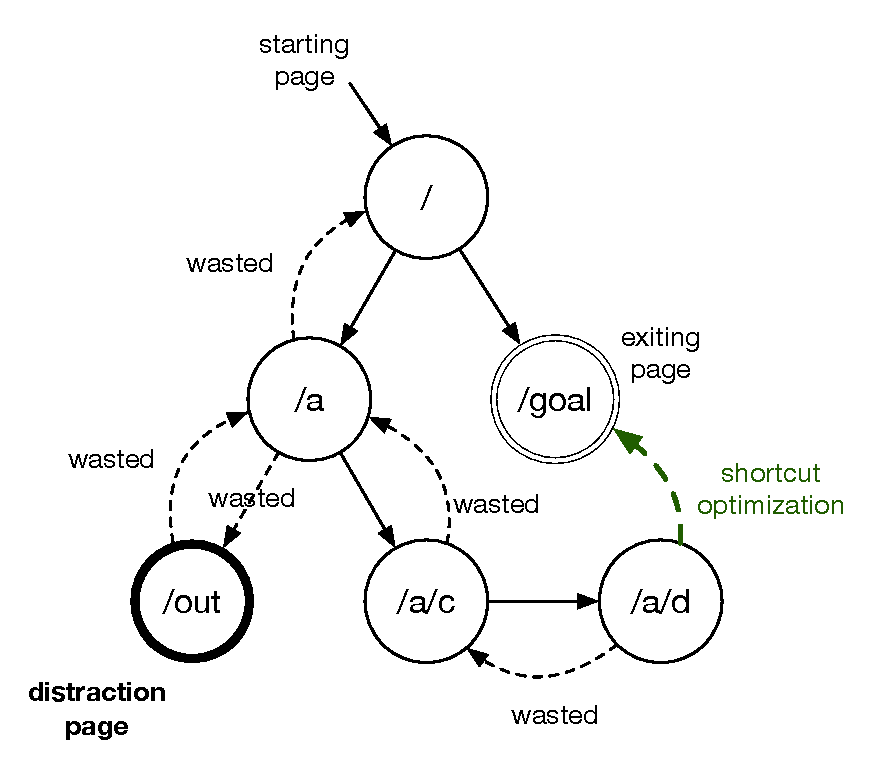
\includegraphics[width=0.5\textwidth]{figures/clickstream}
    \caption{A simple action path. A user starts from the starting page, and performed
    a series of page click actions, ends on a exiting page. 
    The server side records clickstream in the following order:
    / $\rightarrow$ /a $\rightarrow$ /out $\rightarrow$ /a/c $\rightarrow$ /a/d $\rightarrow$ /goal.
    However the actual user actions are: 
    / $\rightarrow$ /a $\rightarrow$ /out $\rightarrow$ /a $\rightarrow$ /a/c $\rightarrow$ /a/d 
    $\rightarrow$ /a/c $\rightarrow$ /a $\rightarrow$ / $\rightarrow$ /goal. 
    The records from server side lost the interaction details between users and browsers.
    Node that /out is a distraction page in the graph, 
    which may located in a different website (e.g. advertisement), 
    and black dashed arrorws are wasted user
    actions. The /goal page may not clear in the beginning of the clickstream, one can generate
    a shortcut optimization navigation to the /goal page while more clickstream context
    be presented, i.e. an optimized user action is 
    / $\rightarrow$ /a $\rightarrow$ /a/c $\rightarrow$ /a/d $\rightarrow$ /goal. In this case,
    the demand page of the visit session is discovered in /a/d.}
    \label{fig:clickstream}
\end{figure}

For the convenience of discussion, \textbf{we mix the use of 
term \emph{action path} and \emph{clickstream} in
this thesis to indicate a chronologically ordered user actions}.

\subsection{Completion Effeciency}

An action path of a visiting session starts from a starting page and ends on an existing page.
Since we consider the effect of browser back button and browser tab switches, 
a previous page could easily be visited twice, if a user clicked the back button. 
Therefore, a page may direct to multiple pages. \emph{For instance, 
an action path can degrade to a linked list if the user clicks through different pages 
without using the back button and switching tabs; or an action path can become 
a 1-to-n bipartite graph if a user use back button back to the previous page after 
clicking a page or only switching tabs from a specific page to one another}, 
as shown in Figure \ref{fig:sim-action-path}.

As a result, we define a term \emph{completion effeciency} based on shortest path from 
starting page to exiting page, and stay duration of the action path. 

\begin{figure}[H]
    \centering

\begin{subfigure}[b]{0.55\textwidth}
    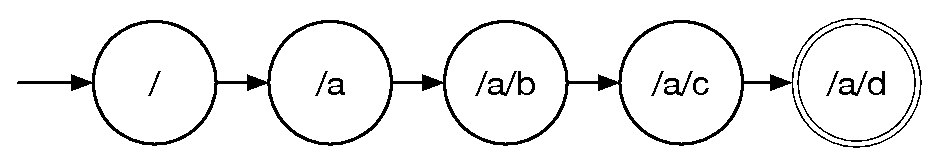
\includegraphics[width=1\textwidth]{figures/linked-list}
    \caption{}
    \label{fig:sim-action-1}
\end{subfigure}
    
\begin{subfigure}[b]{0.23\textwidth}
    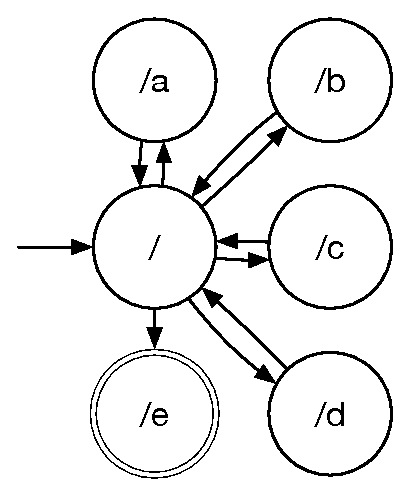
\includegraphics[width=1\textwidth]{figures/1ton}
    \caption{}
    \label{fig:sim-action-2}
\end{subfigure}

\caption{Two particular case of an action path: an action path that degrade to 
a linked list if the user click through different pages without using back button and 
switching tabs (\ref{fig:sim-action-1}), and an action path that represented 
in 1-to-n bipartite graph if a user use back button back to the previous page after 
clicking a page or only switching tabs from a specific page to one another (\ref{fig:sim-action-2}).}
\label{fig:sim-action-path}
\end{figure}

Let a directed cyclic graph represents an action path, each node represents a visited page, 
and each edge has a weight that represents the study duration of its tail node.
Assume the total stay duration of the shortest path from the starting page to 
the existing page is $d_s$, and the total stay duration of the action path is $D$, 
the number of nodes in the shortest path is $n_s$, the total nodes in an action path is $N$, 
we define the \emph{completion efficiency $E$} is as follows Equation \ref{eqn:completion-effeciency}:

\begin{align}
\label{eqn:completion-effeciency}
\begin{split}
    E = w_1 \frac{n_s}{N} + w_2 \frac{d_s}{D}\\
    w_1 + w_2 = 1
\end{split}
\end{align}

where $w_1$, $w_2$ are hyperparameters to balancing the importance of action path and 
stay duration. According to the discussion of two special cases of action path, 
it is trivial to show the range of $E$ is $(0, 1]$. As a compliment, we define 
\emph{zero completion efficiency} if and only if a user cannot complete a clickstream 
in a browsing session. Therefore we have a range of $E$ is $[0, 1]$.

\paragraph{Remark 1} The definition of completion efficiently uses the term of shortest path,
which is the problem of finding a path between the starting page and exiting page 
in an action path (directed cyclic graph) such that the sum of the stay duration of 
its constituent pages in minimized.
The problem can be solved by Dijkstra's \cite{dijkstra1959note} shortest-path algorithm. 
It selects the unvisited nodes with the smallest weights, calculates the distance 
through it to each unvisited neighbor, then updates the distance of neighbor distance 
if the distance is smaller than one another. The process converges to the shortest path.

\paragraph{Remark 2} An action path may increases with more nodes (web pages) over time.
The starting page of an active path was always the first page when the browser was opened.
However, one can always treat the currently visited page is the exiting page due to we
do not know when a user will exit browsing overtime at the moment. 
Consequently, function $E$ is changing over browsing.

\paragraph{Remark 3} We use completion efficiency as a feature for a classification task 
in Section \ref{sec:inter-general-feature}.

\subsection{\emph{url2vec} Embedding}

As we discussed in Section \ref{sec:seq-learn}, we convey similar idea from word2vec model 
and propose our \emph{url2vec} model for client side clickstream data.

The purpose of url2vec model is to construct URL representations that better predict 
the surrounding URLs in a clickstream. Briefly, given a clickstream of urls 
$\text{URL}_1, \text{URL}_2, ..., \text{URL}_T$, the objective of url2vec is to maximize 
the average log softmax probability:

\begin{align}
\label{eqn:url2vecprob}
\begin{split}
    \frac{1}{T}\sum^{T}_{t=1}\sum_{-c \leq i \leq c, i \neq 0} {\log{p(\text{URL}_{t+i} | \text{URL}_t)}}\\
    p(\text{URL}_{t+i} | \text{URL}_t) = \frac{
        \exp{(v_{\text{URL}_{t+i}} ^\top v_{\text{URL}_t})}
    }{
        \sum_{\text{all URLs}} {\exp{(v_{\text{URL}_{t+i}} ^\top v_{\text{URL}_t})}}
    }
\end{split}
\end{align}

where $c$ is the size of embedding context, which is a function of starting page,
$v_{\text{URL}_t}$ is one-hot encoded representation of input URLs, and 
$v_{\text{URL}_{t+i}}$ is the vector embedding of output representations.

\paragraph{Remark 1} The model described by Equation \ref{eqn:url2vecprob} is essentially
a three layer neural network: input layer of \emph{one-hot} encoded URLs (a group of binaries
that a component of a one-hot encoded vector is a representative of a URL under a finite set
of existing URLs), a hidden layer of feature representation and an output layer 
share weights to the learned embeddings of input URLs.

\paragraph{Remark 2} The probability in Equation \ref{eqn:url2vecprob} is impractical due to
$\nabla \log{p(\text{URL}_{t+i} | \text{URL}_t)}$ is large because of exponential terms in softmax,
two numerical optimizations \cite{mikolv2013embedding} based on Hofmann Tree and Negative Sampling
are proposed by Mikolv.

\paragraph{Remark 3} The probability can also be interpreted from a Bayesian perspective,
which provides an intuition of this definition. $p(\text{URL}_{t+i} | \text{URL}_t)$
can be considered as a posterior probability. Since $v_{\text{URL}_t}$ was initialized
as a one-hot encoded vector input to the embedding neural network, the item can be treated
as a prior, and the denominator is a normalization term.
Furthermore, the dot product between $v_{\text{URL}_{t+i}} ^\top$
and $v_{\text{URL}_t}$ is a representation of consine similarity, which represents
the closest surrounding URLs in same direction of vectors.

\subsection{Action Path Model}

Our model convey a similar idea from Stutskever's sequence 
to sequence translation as we discussed in Section \ref{sec:seq-learn}.

An \emph{action path} from user $i$ in session $j$ consist of 
a sequence of \emph{url2vec} embedded vectors $(U^{ij}_1, U^{ij}_2, ..., U^{ij}_n)$ 
and a sequence of time duration $(d^{ij}_1, d^{ij}_2, ..., d^{ij}_n)$, since each URL 
has a corresponding number that represents the time duration of a user spent on a given page.
Our action path model consist a context encoder and a context decoder that illustrated in the subsequent
subsections.

\subsubsection{Context Encoder}

\emph{Context encoder} encodes URLs one by one over timestamp and produces a context tensor 
that encodes the historical user actions, as shown in Figure \ref{fig:encoder}. 

In the encoder, we practically insert a starting mark (a mark is a special URL vector that 
differ from any other realistic URL one-hot encoded vectors) ``<SOA>'' (\emph{Start of Action})
as a sign of start feeding URLs to the encoder, and a trigger mark ``<COI>'' (\emph{Change of Intention}) as
a sign to trigger decoder to decodes encoded context tensor.

\begin{figure}
    \centering
    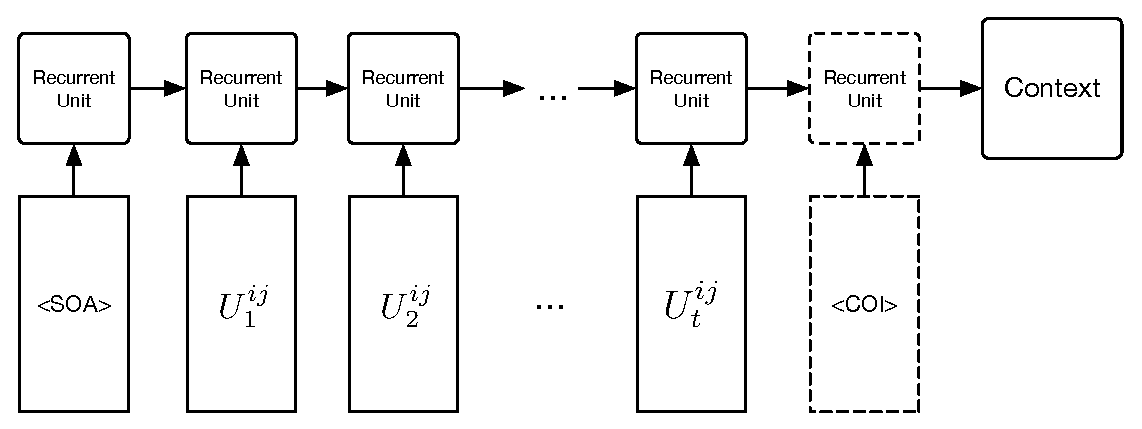
\includegraphics[width=0.7\textwidth]{figures/encoder}
    \caption{An unrolled illustration of context encoder of Action Path Model. 
    In the encoder, a starting mark ``<SOA>'' is used as a sign of start feeding URLs, 
    and a trigger mark ``<COI>'' as a sign to trigger decoder to decodes 
    encoded context tensor. The trigger mark is automatically inserted after the $k$-th URL 
    while training at the end of the encoder model over time, $k$ is increasing over time. 
    Besides, the recurrent unit is not detailly described in the figure but afterward.}
    \label{fig:encoder}
\end{figure}

Note that the input URLs to encoder's recurrent unit are preprocessed through 
url2vec embeddings, which has learned and updated from one-hot encoded vectors to 
densely distributed vectors.

\subsubsection{Context Decoder}

\emph{Context decoder} decodes the context tensor produced by the encoder into a series of URLs. 
We practically feed a prediction mark ``<SOP>'' (\emph{Start of Prediction}) 
as a sign to initiate the decoding of encoded context. 
At the end of decoder, decoder produces an ending mark ``<EOA>'' (\emph{End of Action}) 
that terminates the decoding process.

Note that the decoder model in the training phase and prediction phase is different.
In the training phase, teacher forcing strategy \cite{williams1989learning} is used, 
the strategy supplies observed user actions as inputs in the decoder.
In the evaluation phase, the decoder uses the output from the recurrent unit as an input, 
shown through dashed lines in Figure \ref{fig:decoder}.

\begin{figure}
    \centering
    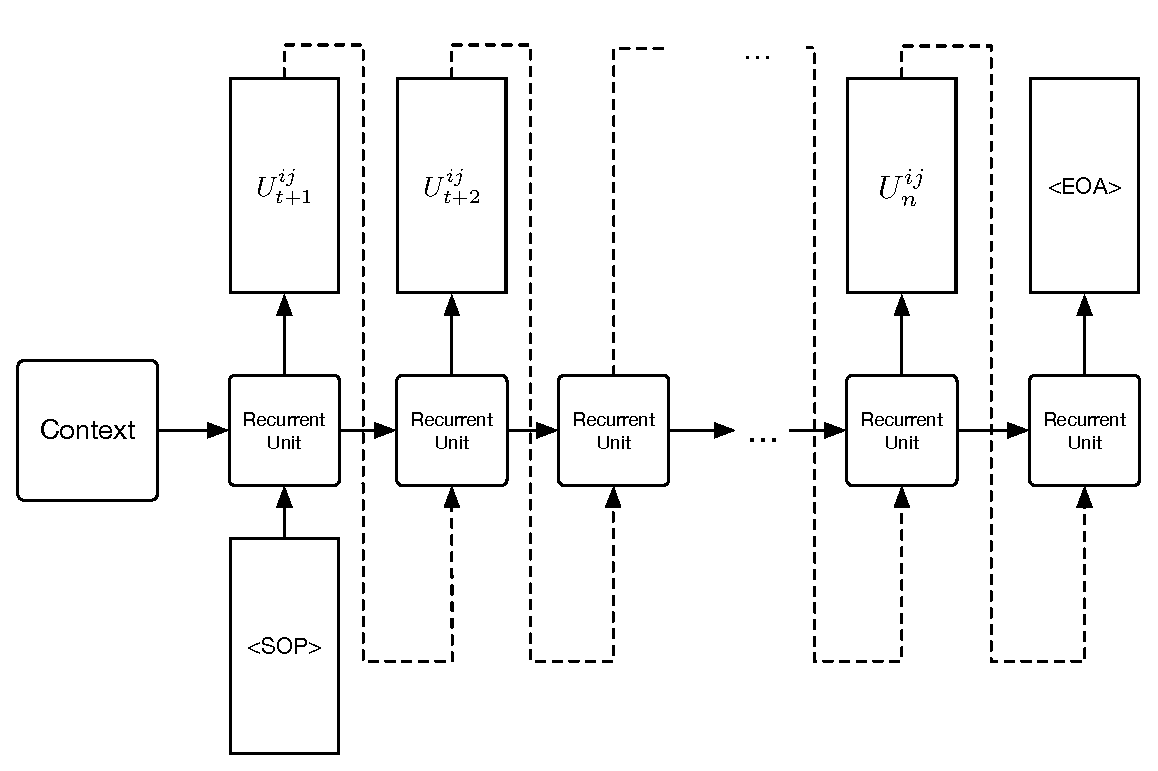
\includegraphics[width=0.7\textwidth]{figures/decoder}
    \caption{The context decoder of the Action Path Model. In the decoder, 
    a prediction mark ``<SOP>'' is used to initiate the decoding process, 
    and an ending mark ``<EOA>'' as a sign to terminate decode process. 
    The output of the decoder uses a softmax intermediate operation to magnify 
    and normalize the probability of predicted URL embedding. Also, the recurrent unit 
    is not detailly described in the figure but afterward.}
    \label{fig:decoder}
\end{figure}

In our model, a decoder outputs vectors first, and we have two strategies 
in translating vectors to URLs. 
The first strategy is to use an argmax function to select the component 
with maximum probability of a vector; we use this strategy for performance evaluation 
in Section \ref{sec:eval-optimal}. Another strategy is to select a series of URLs 
that gains the highest joint probability,  we discuss and use this strategy 
for action path optimization in Section \ref{sec:optimization}.

\subsubsection{Recurrent Unit}
\label{sec:recurrent-unit}

\textbf{The recurrent unit in the Action Path model is not as standard as original 
LSTM or GRU}, which is one of the major contributions of the thesis. 
In our recurrent unit, when using LSTM as recurrent unit base, we also 
feed time duration $(d^{ij}_1, d^{ij}_2, ..., d^{ij}_n)$
into input gate $I_t$, and others (forget gate $F_t$, output gate $O_t$, 
memory cell $C_t$ and hidden state $h_t$) remains the same:

\begin{align}
\label{eqn:lstm}
\begin{split}
    I_t =& \sigma ( P^{(I)} U^{ij}_t + Q^{(I)} h_{t-1} + \frac{d^{ij}_t}{d^{ij}_t + 1}) ) \\
    F_t =& \sigma ( P^{(F)} U^{ij}_t + Q^{(F)} h_{t-1} + b^{(F)}) \\
    O_t =& \sigma ( P^{(O)} U^{ij}_t + Q^{(O)} h_{t-1} ) \\
    C_t =& F^{(t)} \circ C_{t-1} + I_t \circ \tanh (P^{(C)} U^{ij}_t + Q^{(C)} h_{t-1}) \\
    h_t =& O_t \circ \tanh (C_t)
\end{split}
\end{align}

where $t = 1, 2, ..., n; P^{(I)}, Q^{(I)}, P^{(F)}, Q^{(F)}, P^{(O)}, Q^{(O)}$ are shared weight parameters, 
$b^{(F)}$ is a bias in forget gate $F_t$,
$\circ$ represents element-wise product of two matrices.

When using GRU as recurrent unit base, we feed time duration $(d^{ij}_1, d^{ij}_2, ..., d^{ij}_n)$
in to update gate $Z_t$, and others (reset gate $R_t$, hidden state $h_t$) stay the same:

\begin{align}
\label{eqn:gru}
\begin{split}
    Z_t =& \sigma ( P^{(Z)} U^{ij}_t + Q^{(Z)} h_{t-1} + \frac{d^{ij}_t}{d^{ij}_t + 1} ) \\
    R_t =& \sigma ( P^{(R)} U^{ij}_t + Q^{(R)} h_{t-1} ) \\
    h_t =& ( 1 - Z_t ) \circ \tanh ( P^{(H)} U^{ij}_t + Q^{(H)} h_{t-1} ) + Z_t \circ h_{t-1}
\end{split}
\end{align}

where $t = 1, 2, ..., n; P^{(Z)}, Q^{(Z)}, P^{(R)}, Q^{(R)}, P^{(H)}, Q^{(H)}$ are shared weight parameters, 
$\circ$ represents element-wise product of two matrices.

\paragraph{Remark 1} The units we described in this section is neither LSTM nor GRU since
the input gate $I_t$ or update gate $Z_t$ introduces time duration $d^{ij}_t$ as input,
which is different from a simple constant bias in the first learnable bias in these gates. 
It is worth mentioning that adding bias to the gates are helpful to 
improve learning performance in LSTM \cite{Jozefowicz:2015:EER:3045118.3045367}, 
we also use the trick in our model as shown in $F_t$ of Equation \ref{eqn:lstm}.

\paragraph{Remark 2} The term $\frac{d^{ij}_t}{d^{ij}_t + 1}$ is a squashing mechanism,
it normalizes $d^{ij}_t$ from $(0, \infty)$ to $(0, 1)$.

\subsubsection{Ending Mark Interpretation}
\label{sec:mark-interpretation}

In context decoder, we mentioned an ending mark ``<EOA>'' that indicates the 
termination decoding process. However, the ending mark is different from other marks, 
since in practice, ``<EOA>'' is represented in different symbols of 
behavior-based categorical clickstream, which as a label to 
involve classification of user actions.

Assume action paths are labeled by one-hot encoded ending marks 
$\text{EOA}_1, \text{EOA}_2, ..., \text{EOA}_m$ and the last output
of decoder hidden state is $h_n$, we have:

\begin{align}
\label{eqn:mark}
\begin{split}
    \hat{y} =& \text{argmax} (\text{softmax} (W^{(M)} h_n)) \\
    \hat{y} \in& \{ \text{EOA}_1, \text{EOA}_2, ..., \text{EOA}_m \}
\end{split}
\end{align}

where $W^{(M)}$ is a weight parameter, and $m$ is the number of ending mark categories.

\subsection{Action Path Optimization}
\label{sec:optimization}

In traditional classification models, the arguments of the maxima (argmax) are used 
to select labels with the highest probability, scilicet, argmax selects predicted URLs 
with the highest probability of user action from decoder outputs. However, this method 
is under the condition of all outputs are independent in probability, which 
is not suitable for our action path optimization scenario.

In previous sections, our model feeds an input clickstream $(U^{ij}_1, U^{ij}_2, ..., U^{ij}_t)$,
and produce an output $(o_1, o_2, ..., o_{m})$ that expect close to actual clickstream 
$(U^{ij}_{t+1}, U^{ij}_{t+2}, ..., U^{ij}_n)$.
Then the probability of expected clickstream is a conditional probability under 
the input clickstream. In other words, we need to solve an optimization problem:

\begin{align}
\label{eqn:optimize}
\begin{split}
    & \operatorname*{argmax}_{o} p( o_1, o_2, ..., o_{m} | U^{ij}_1, U^{ij}_2, ..., U^{ij}_t ) \\
   =& \operatorname*{argmax}_{o} \prod_{k=1}^{m} p(o_{k} | U^{ij}_1, ..., U^{ij}_t, o_1, ..., o_{k-1}) \\
   =& \operatorname*{argmax}_{o} \sum_{k=1}^{m} \log p(o_{k} | U^{ij}_1, ..., U^{ij}_t, o_1, ..., o_{k-1})
\end{split}
\end{align}

A heuristic approach can solve the optimization problem efficiently, namely beam search 
\cite{DBLP:journals/corr/abs-1211-3711}.
In each step of decoder output, we reserve the top-$k$ best combinations of URLs and 
eliminate the rest of URLs from evaluation, and finally selects $k$ best clickstreams.
The pseudocode is given that adapts vanilla beam search to URL prediction search 
in Algorithm \ref{algo:optimize}.

~\\

\begin{algorithm}[H]
\label{algo:optimize}
\SetAlgoLined
\SetKwInOut{Input}{input}\SetKwInOut{Output}{output}
\Input{Decoder outputs $(o_1, o_2, ..., o_{m})$,\\
        Number of candidates $k$}
\Output{k clickstream candidates with highest probability}
\Begin{
    Initialize empty $\text{clickstreams}$ list \\
    \For{$o$ $\in$ $(o_1, o_2, ..., o_{m})$}{
        Initialize empty $candidates$ list \\
        \For{$\text{clickstream}$ $\in$ $\text{clickstreams}$}{
            \For{page $\in$ $o$)}{
                candidates.append([clickstream.append(page), $log(p(\text{clickstream})) + log(p(\text{page}))$]) \\
            }
        }
        ordered = descending order sort candidates by score \\
        clickstreams = ordered[:k]
    }
}
\caption{Output Clickstream Search}
\end{algorithm}

~\\

\paragraph{Remark} The algorithm produces a heuristic output with given clickstream context. 
Combining with the \emph{url2vec} model, the prediction
can heuristically optimize the click path of a specific user since the embeddings 
are trained over all possible action path. For instance, 
a distraction advertisement page will not appear
after optimization because the embedding of the advertisement page 
is far from the desired page if embeddings are learned correctly.

\cleardoublepage
\section{Experiment}
\label{ch:exp}

In this chapter, we rationalize the process of our lab study based on the theory of
human information behavior, then construe 
the purpose of context given web browsing tasks to our subjects.

The lab study took place during the last two weeks of November, from 14/11/2018 to 29/11/2018
in Frauenlobstrasse 7a, a faculty building of Ludwig-Maximillians-Universitaet Muenchen.
Client-side user clickstream data was collected by a embedded collector plugin installed in 
the mainstream browser, i.e. Google Chrome, on a self provided desktop computer and a laptop.

In lab study, we select three mainstream websites, Amazon/Medium/Dribbble, 
that covers categories for shopping, media consuming and design brainstorming with design 
reasons (discuss later in Section \ref{sec:task-design}).
Then we manually designed 35 reasonable tasks and finally selected 9 
context-given browsing tasks (three for each website, discuss in 
Section \ref{sec:task-design}) to simulate three different proposed browsing behavior,
namely goal-oriented/fuzzy/exploring behaviors.
Each task requires participant start from a starting page of a given website, and
all tasks do not restrict participants use the given website, but also allow they 
access websites outside the landing page to help they complete the task (explicitly informed to 
participants before participation).
Participants start browsing after they completely understand the requirements of 
each task, and no interruption or question answering during the task
except exceeding time limit of a task, however subjects can either acquire more time 
to accomplish the task or give up directly.

The study is designed as a within-subject study, thus every participant performs all tasks. 
To eliminate the learning effect due to the long time of using same websites, 
we use Latin square \cite{cochran1950experimental} 
for the device (Desktop/Laptop) and tasks participation order to our participants.

Our lab study obtained 21 participants with a mean age of 23.04 (standard deviation of 3.216, min=18 and max=19) 
took part in the study, 10 male and 11 female, whom are recruit anonymously and 
randomly via a mailing list.

\subsection{Environment}

The lab study uses two self provided devices: a desktop computer and a mobile laptop.
The reason of choose two morphology of computing device is our study requires recording
a complete clickstream of during the study.

A major issue of mobile devices is the operating system installed in mobile phone does not
authorize the permission of allowance to collect data precisely over pages or user actions.
Though Android device can overpass system permission to privilge, the user behavior 
between iOS and Android device has different personalities \cite{sandoio2018android}, and subjects shows \cite{reinfelder2014androidios} abnormal awareness behavior regarding security and privacy issues when they handling a newly provided Android device when switch from iOS device.
Therefore, to eliminate this awareness, we stick our study environment to desktop devices,
which empower us easily collects the clickstream data from browsers with plugin supports.

Although all modern browsers support plugin development, considering the usage share of 
all browsers on the market, Google Chrome \cite{wiki2018share} obtains 61.7\% 
market shares of desktop browsers, and Apple Safari only shares
15.0\% of the market. Clearly, Google Chrome dominant market of the desktop web browser.

Hence, we decide to use Chrome to establish our plugin of data collection.
The quesionaire after our lab study indicates the browsers usage share of all subjects, 
as shown in Table \ref{table:sharesubjects}, which further supports our decision of 
browser selection.

\begin{table}[H]
    \small
    \centering
    \setlength{\belowcaptionskip}{10pt}
    \caption{Browser Usage Shares of Lab Study Subjects}
    \begin{tabular}{ccccc}
          \toprule
        & \textbf{Google Chrome} & \textbf{Apple Safari} & \textbf{Mozilla Firefox} & \textbf{Microsoft Edge} \\
          \hline
          Number     & 11 & 5 & 3 & 2 \\
          Percentage & 52.38\% & 23.81\% & 14.29\% & 9.52\% \\
          \bottomrule
    \end{tabular}
    \label{table:sharesubjects}
\end{table}

% \subsection{Context-given Websites}

% In our study, we gathered various websites covering most of the categories that people do
% on the Internet: Social Networks, Shopping, Email, Media Consuming, Search, Production 
% and etc \cite{lori2018internet, lori2017internet}. All selected website are listed 
% in Table \ref{table:websites}.

% \begin{enumerate}
%     \item social network: facebook / twitter / weibo
%     \item shopping: amazon.com / ebay.com
%     \item search: google.com / bing.com / baidu.com
%     \item media: medium.com
%     \item development: github.com
%     \item design dribbble.com
%     \item study medien.ifi.lmu.de
%     \item study en.uni-muenchen.de
%     \item streaming media youtube.com
%     \item research arxiv.com
%     \item study ielts.org
%     \item media bloomberg.com/europe
%     \item social community reddit.com
% \end{enumerate}

% \begin{table}[H]
%     \small
%     \centering
%     \setlength{\belowcaptionskip}{10pt}
%     \caption{Browser Usage Shares of Lab Study Subjects}
%     \begin{tabular}{ccccc}
%           \toprule
%         & \textbf{Google Chrome} & \textbf{Apple Safari} & \textbf{Mozilla Firefox} & \textbf{Microsoft Edge} \\
%           \hline
%           Number     & 11 & 5 & 3 & 2 \\
%           Percentage & 52.38\% & 23.81\% & 14.29\% & 9.52\% \\
%           \bottomrule
%     \end{tabular}
%     \label{table:sharesubjects}
% \end{table}

% \subsection{Pilot Study}

% Initially, we developed a web crawler that downloaded the entire medien computer science website 
% \footnote{\url{https://medien.ifi.lmu.de}}
% .... TODO discuss how we go here?


\subsection{Browsing Behaviors}
\label{sec:behavior}

Before we explain the design reason of our context-given browsing task, 
we first present and discusses three common types of user browsing process as behavior: \textbf{goal-oriented}, 
\textbf{exploring} and \textbf{fuzzy}.

These three terminologies are aggregated and incorporated from behaviors that concluded 
in former qualitative research for web browsing behavior research, 
all these terminologies are based on a fundmental theory of 
interdisciplinary perspective information seeking behavior \cite{wilson1997information},
which was discussed in Section \ref{sec:info-seek}.
Table \ref{table:info-seek} compares the terminology differences between former research and our thesis.

\begin{table}[H]
    \small
    \centering
    % \setlength{\belowcaptionskip}{10pt}
    \caption{Terminologies comparison of information behavior on the web}
    \begin{adjustbox}{width=\textwidth}
        \begin{tabular}{ccccc}
            \toprule
            \textbf{Author} & \textbf{Terminologies} & \textbf{Terminologies} & \textbf{Terminologies} & \textbf{Main Factors} \\
            \hline
            \cite{choo1999information} & Formal search & \makecell{Conditioned viewing; \\ Informal search} & Undirected viewing & \makecell{Psychological; demographic;\\ role-related environmental; \\source characteristics} \\
            \cite{johnson2017patterns} & \makecell{Directed browsing; \\Known-item search} & \makecell{Semi-directed browsing; \\Explorative seeking; \\``You do not know what you need''; \\Re-finding} & Undirected Browsing & Behavior \\
            \textbf{This thesis} & \textbf{Goal-oriented} & \textbf{Fuzzy} & \textbf{Exploring} & \textbf{Purpose} \\
            \bottomrule
        \end{tabular}
        \label{table:info-seek}
    \end{adjustbox}
\end{table}

To justify our terminology, we combines the six qualitative activities from Ellis' Model 
\cite{ellis1989behavioural} and ``information use'' in information behavior theory 
to represent our summarized browsing behaviors:

\paragraph{Goal-oriented behavior} occurs when a user initiate 
visiting session on the web caused by a determined objective in a specific context, 
such as bussiness work, 
social communication, university study, literature research and etc. 

Goal-oriented behavior indicates an actively information seeking behavior.
Instead of \emph{formal search}, that only covers the phase of ``monitoring'' and ``extracting''
(or \emph{directed browsing} and \emph{known-item search} that covers ``browsing'' and ``differentiating'' or 
``monitoring'' and ``extracting'' respectively), 
goal-oriented browsing behavior contains the entire life cycle of human information behavior starts
from ``starting''. Under browsing behavior, a determined ``information use'' can be observed
or concluded.

For instance, a college student intentionally need a latest lecture slide (\emph{information use} observed), 
the student then opens web browser, access college website (\emph{starting}) and navigates to the lecture homepage 
(\emph{chaining}, \emph{browsing}, and \emph{differentiating}).
Finally, the student exit browsing after download the slides (\emph{monitoring} and \emph{extracting}).

\paragraph{Exploring behavior} occurs when a user initiates browsing session aimlessly with no clear observed
extracting or information use during the session, the person greedily or breadth-first consumes and the content on the Web without 
any information extracting and information use, such as media consuming, learning before using and etc.

Exploring browsing behavior indicates a complete opposite behavior comparing to 
goal-oriented borwsing behavior. More formally describing exploring behavior using Ellis' model, 
the behavior represents ``chaining'' and ``browsing''
without ``differentiating'' and ``extracting'' from ``starting'' while information seeking.

For instance, a person who accesses an unknown utility web application (\emph{starting}), he/she explores
what functions are provided one by one and what he/she can do while using the application
(\emph{chaining} and \emph{browsing}).

\paragraph{Fuzzy behavior} occurs when a user initiate visiting session for information use
 with non-systematic, incomplete prior knowledge that may browsing ongoing for updating 
the framework of knowledge until final acquisition or abandon.

Fuzzy behavior in a browsing behavior in between of goal-oriented and exploring behaviors.
Instead of only ``chaining'' and ``browsing'' from ``starting'', fuzzy behavior also do
``differentiating'' or ``monitoring'' while information seeking.

For instance, a researcher heared a new technique proposed in another scientific field 
that may influence he/she's research, then the person 
opens a search engine (\emph{starting} and \emph{chaining}) to seek (\emph{browsing}) existing (\emph{differentiating}) 
follow up researches (\emph{monitoring}). The browsing may ends without information use
because of the technique is irrelevant to he/she's research.

\paragraph{Remark} Table \ref{table:ellis} illustrates the exist activities of our three
browsing behavior. Note that ``information needs'' is not suggested in Wilson's theory \cite{wilson1981user} 
since ``information needs'' can not be clearly observed before information seeking but sometimes
observed after information use. Therefore we do not take information need into the 
consideration of our terminologies.

\begin{table}[H]
    \small
    \centering
    % \setlength{\belowcaptionskip}{10pt}
    \caption{Existence of activities from Ellis' Model and information use in 
    goal-oriented, exploring and fuzzy browsing behavior}
    \begin{adjustbox}{width=\textwidth}
        \begin{tabular}{ccccccccc}
            \toprule
            \multicolumn{1}{c}{\multirow{2}{*}{\textbf{Behaviors}}}  & \multicolumn{1}{c}{\multirow{2}{*}{\textbf{Information Need}}} & \multicolumn{6}{c}{\textbf{Information Seeking}}                                    & \multicolumn{1}{c}{\multirow{2}{*}{\textbf{Information Use}}} \\ \cline{3-8}
            \multicolumn{1}{c}{}                                     & \multicolumn{1}{c}{}                                  & \textbf{Starting} & \textbf{Chaining} & \textbf{Browsing} & \textbf{Differentiating} & \textbf{Monitoring} & \textbf{Extracting} & \multicolumn{1}{c}{}  \\
            \hline
            Goal-oriented                                            &   N/A                                                 &     Exist         &      Exist        &   Exist           &        Exist               &       Exist           &        Exist          &      Exist              \\
            Exploring                                                &   N/A                                                 &     Exist         &      Exist        &   Exist           &        Exist               &       Exist           &                     &                       \\
            Fuzzy                                                    &   N/A                                                 &     Exist         &      Exist        &   Exist           &                          &                     &                     &                       \\
            \bottomrule
        \end{tabular}
        \label{table:ellis}
    \end{adjustbox}
\end{table}

\subsection{Tasks Design}
\label{sec:task-design}

We designed 35 browsing tasks, after conduct a pilot study, 
9 tasks are selected for three websites: Amazon.com, Medium.com and Dribbble.com 
because of the following reasons:

\begin{enumerate}
    \item These three websites all have coresponding tasks to the three type of browsing behavior;
    \item Each of the task can be finished around 5 to 10 minutes;
    \item All these websites are mainstream websites, they do not require 
        massive professional domain knowledge for using.
\end{enumerate}

In addition, the unselected tasks are listed in Appendix \ref{appendix:unselected}.

\subsubsection{Goal-oriented Task}

We designed and selected an appropriate goal-oriented task for selected websites respectively,
and each task is designed with three specifically designed information need as
the cause of information use.

\paragraph{Amazon.com} \emph{Assume your smartphone was broken and you have 1200 euros 
    as your budget. You want to buy an iPhone, a protection case, and a wireless 
    charging dock. Look for these items and add them to your cart.}

This task initiate from the homepage of Amazon (\emph{starting} and \emph{chaining}), 
and it contains three determined objective since 
a subject is required to add three specific items to the cart (\emph{information use}). 
There are few hidden consideration behind the task (\emph{browsing} and \emph{differentiating}),
which makes the task more realistic (\emph{monitoring} and \emph{extracting}): 
a) There is a budget of this task, which requires subjects must consider the
price of items instead of simply add the first recommended item to cart; 
b) the starting page is amazon.com instead of amazon.de. This decision requires
subjects must also consider the currency rate between US dollars and Euros for budget.
c) There are some items cannot be shipped to Germany (the study took place in Germany).
As a result, subjects cannot add these items to cart and they should find other alternatives.

\paragraph{Medium.com} \emph{Assume you were making plans for your summer vacation. 
        You want to visit Tokyo, Kyoto, and Osaka. You want to find out what kind of experience other people made 
        when traveling to these three places in Japan. Your task is to find three posts 
        for traveling tips regarding these cities. Elevate a post if it is one of your choices.}

This task contains three determined purpose since there are three fixed traveling destination.
The task also implies few considerations that increase the required interaction of the task to subjects:
a) The website only offers English version, some Japanese character may appear in an article,
thus, a translation util may be used while the study;
b) An article may apears numerous noun, such as toponym. Search engine may used while the study;
c) the articles, those require a membership to unlock reading, cannot be elevated. 


\paragraph{Dribbble.com} \emph{You are hired to a Cloud Computing startup company. You get an assignment to 
        designing the logo of the company. Search for existing logos for inspiration and 
        download three candidate logos you like the most.}

The task also has three determined prupose since subjects are quired to download three candicate trademarks.
While the participation, subjects still need take few implicit facts in to account:
a) Subjects who unfamiliar with the term "Cloud Computing" need visit other explainations to figure out
the vision and mission of this type of company, and subjects whom already familiar with the term
still need to compares the designed made by other competitors.
b) Subjects should aware some of the designs shared on the website are not suitable for trademark or icon design.

\subsubsection{Exploring Task}

Exploring tasks simply do not provides any deterministic objective,
and all websites has a designed exploring task for subjects.

\paragraph{Amazon.com} \emph{Look for a product category that you are interested in and start browsing. 
        Add three items to your cart that you would like to buy.}

Although the task do not require any specific items to the subjects, the task remains three different
purpose because participants need add three items to the cart. This designed task 
is aimlessly because: all tasks is not formerly informed to participants, 
they either do not have needs of buying items or 
formerly exist needs of buying a specific category but do not have a product candicate yet.
Besides, the description of the task ask participants start from a product category, which avoids 
goal-oriented buying a specific product.

\paragraph{Medium.com} \emph{Visit a category you are interested in and elevate three post you like.}

Similar reason as discussed in Amazon.com's exploring task. It is well to be remined that Medium is a media
website, visiting a specific article formerly read before participation is relatively difficult 
since all contents showed to users are daily updated. Thus the task can be directly consider as an exploring task.

\paragraph{Dribbble.com} \emph{Explore dribbble and download three images you like the most while you browse.}

Dribbble illustrates designs by using image gallery. The major difference between Dribbble and Google Image Search
is dribbble is a user-centered content aggregation website, but Google Image Search is a simple content aggregation engine.
As a result, there will be two different interaction in Dribbble: exploring designs based on keywords and categories,
or exploring designs based on users. The latter can helps its user finding similar designing style.
The task is aimlessly since the task simply describes nothing and completely let participants explore their preferences.

\subsubsection{Fuzzy Task}

Each of our selected websites also has an fuzzy task respectively, and there are three major goals per task.

\paragraph{Amazon.com} \emph{You want to buy a gift for your best friend as a birthday present.
        Add three items to your cart as candidate.}

The clearness of the task is stronger than exploring task but weaker than goal-oriented task, because
The task restricts participants adding items for a specific purpose (birthday present) but not points
any specific product.

\paragraph{Medium.com} \emph{Assume you got an occasion to visit China for business. 
        You are free to travel to China for a week. 
        You want to make a travel plan for touring China within a week. Your task is to find out what kind 
        of experience other how people made when going to secondary cities or towns in China, then decide 
        on three cities you want to visit (excluding  Beijing, Shanghai, Guangzhou, and Shenzhen). 
        Elevate if a post helped you make a decision.}

The clearness of the task is stronger than exploring task, because it asks a participant 
to exploring a non-deterministic direction of looking for secondary cities.
But the clearness of the task is weaker than goal-oriented task due to secondary cities described
in Medium's user posts is unclear, participants suppose to make decision themselves.
Furthermore, this ask is asking regarding traveling China around a week. Cities cannot be randomly
selected because to make traveling plan requires consider geographic location of the city.

\paragraph{Dribbble.com} \emph{You are preparing a presentation and need one picture for each of these animals: 
    cat, dog, and ant. Download the three pictures you like the most.}

The task has three purpose of downloading images of animals, which restrict participant to a specific direction,
thus, the clearness of the task is stronger than exploring task. However, the task describes a scenario of using
these images in a presentation, and hence participants must consider continuity of design style, which makes
the clearness of the task is weaker than goal-oriented task.

\cleardoublepage
\section{Evaluation}
\label{ch:eval}

In this chapter, we conduct evaluations to our collected data.
The data is collected from 21 subjects, and 189 clickstream data are collected in total. 
Each clickstream contains action-level data with a stay duration
of a specific page, for instance, we still collect an URL as a step of clickstream 
if a participant uses back button rollback to a previous visited page without requesting server. 
A clickstream also has a subjective difficulty score from questionaire (shown in Appendix \ref{appendix:b}) 
after the completion of each task.

\subsection{Subjective Task Difficulty}

This section discusses the subjective task difficulty qualitatively and quantitatively.
Figure \ref{fig:difficulty} illustrates a normalized (raw scores are listed in 
Appendix \ref{appendix:c} Table \ref{table:diff-raw}) subjective difficulty score 
with respect to all tasks.

\begin{figure}[H]
    \centering
    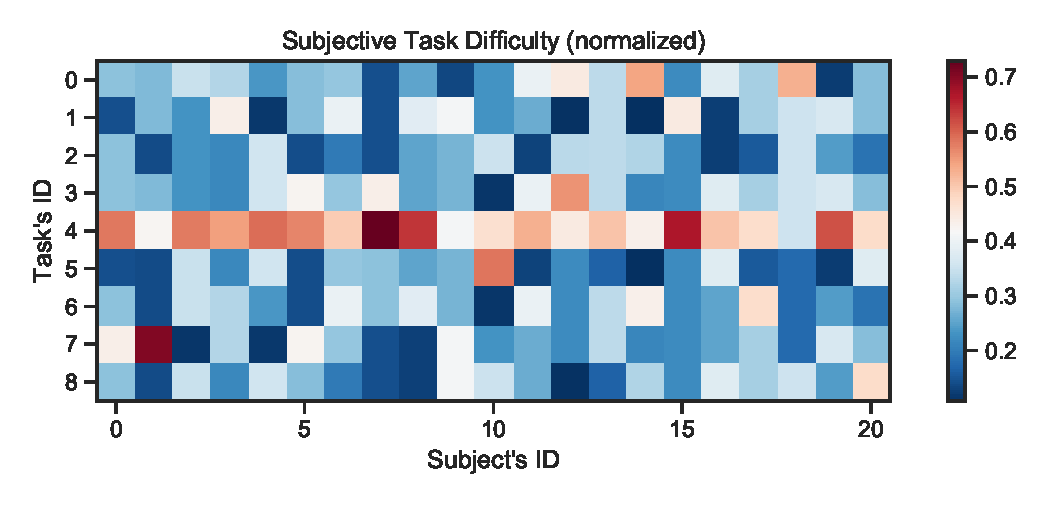
\includegraphics[width=0.7\textwidth]{figures/difficulty}
    \caption{Subjective difficulty score: each column indicates an individual subject and
    each row indicates a browsing task. Tasks from 0 to 8 represent Amazon Goal Oriented Task,
    Amazon Fuzzy Task, Amazon Exploring Task; Medium Goal Oriented Task, Medium Fuzzy Task,
    Medium Exploring Task, Dribbble Goal Oriented Task, Dribbble Fuzzy Task and Dribbble Exploring Task
    respectively.
    From this heat map, we clearly observes Medium Fuzzy Task is the most difficulty task
    according to the subjects voted subjective difficulty, a significant test confirmed this observation.
    Further, Mann-Whitney U significant test justifies our result.}
    \label{fig:difficulty}
\end{figure}

To generalize the task difficulty, the null hypothesis ($H_0$): the difficulty of fuzzy task is not greater
than exploring task and alternative hypothesis ($H_1$): the difficulty of fuzzy task is greater than
exploring task. We conduct non-parametric one-tailed Mann-Whitney U test \cite{mann1947test}, 
under null hypothesis, $p=2.54\times 10^{-5} < 0.05$, reject $H_0$.
Similarly, we compare difficulty score on goal oriented task and exploring task (with corresponding hypothesis, 
$p=0.00534 < 0.05$), difficulty score on fuzzy task and goal oriented task (with corresponding hypothesis, 
$p=0.0145 < 0.05$), all rejects $H_0$. Therefore we concludes the task difficulty is ordered
as follows: \emph{difficulty of fuzzy task $>$ difficulty of goal oriented task $>$ difficulty of exploring task},
which means exploring tasks have lower effort in clickstream, and effort of doing fuzzy task gains highest effort.

\subsection{Browsing Behavior Classification}

As discussed in Section \ref{sec:task-design}, we described three type of browsing behavior. 
In this section, we provides two type of evaluations to interpret the browsing behavior classification.

First, we evaluate the indication of general features browsing behavior,
features including difficulty of task, number of actions in a clickstream as well as the total stay duration in a clickstream.
Then we implements our action path model by using the action-level clickstream data and stay duration of each page,
which was described in Section \ref{sec:recurrent-unit} and \ref{sec:mark-interpretation}.

\subsubsection{Interpretation based on General Features}
\label{sec:inter-general-feature}

% \begin{figure}[H]
%     \centering
%     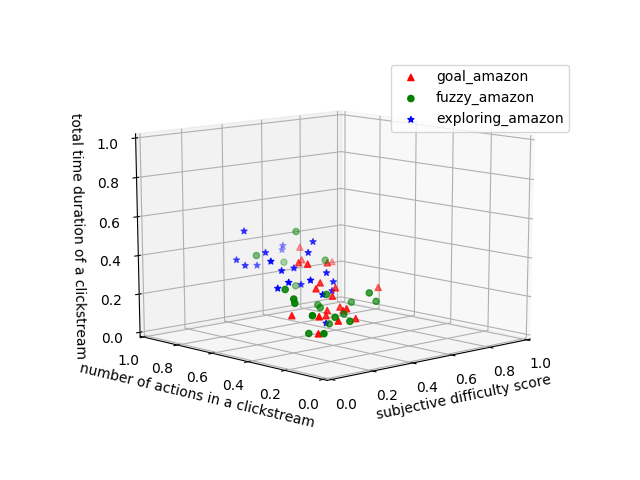
\includegraphics[width=0.49\textwidth]{figures/amazon-general}
%     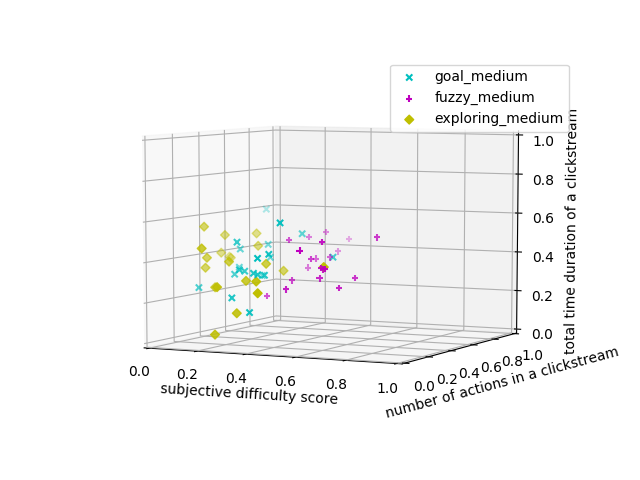
\includegraphics[width=0.49\textwidth]{figures/medium-general}
%     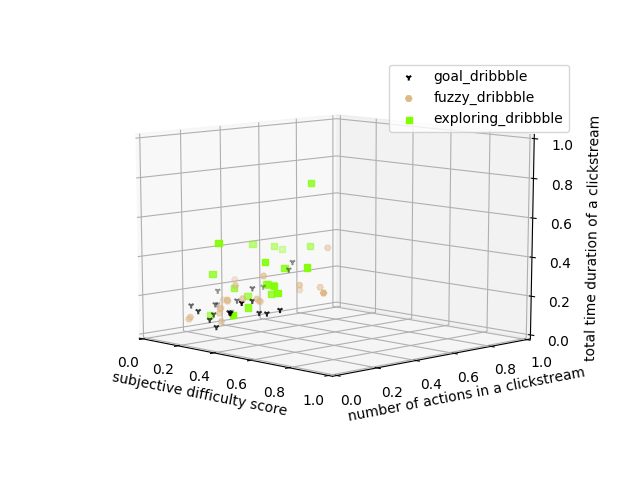
\includegraphics[width=0.49\textwidth]{figures/dribbble-general}
%     \caption{XXXXX}
%     \label{fig:general}
% \end{figure}

\begin{figure}[H]
    \centering
    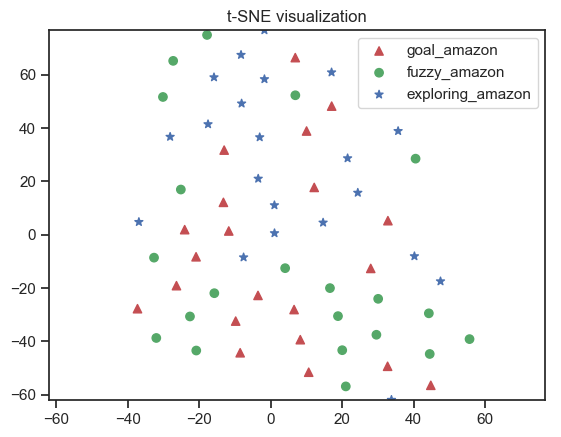
\includegraphics[width=0.25\textwidth]{figures/tsne-amazon}
    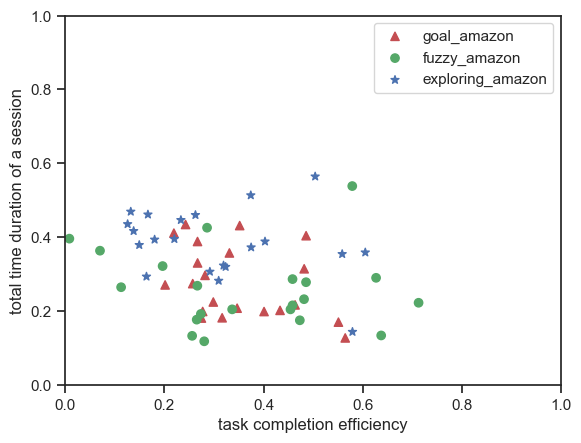
\includegraphics[width=0.25\textwidth]{figures/2d-eff-dur-amazon}
    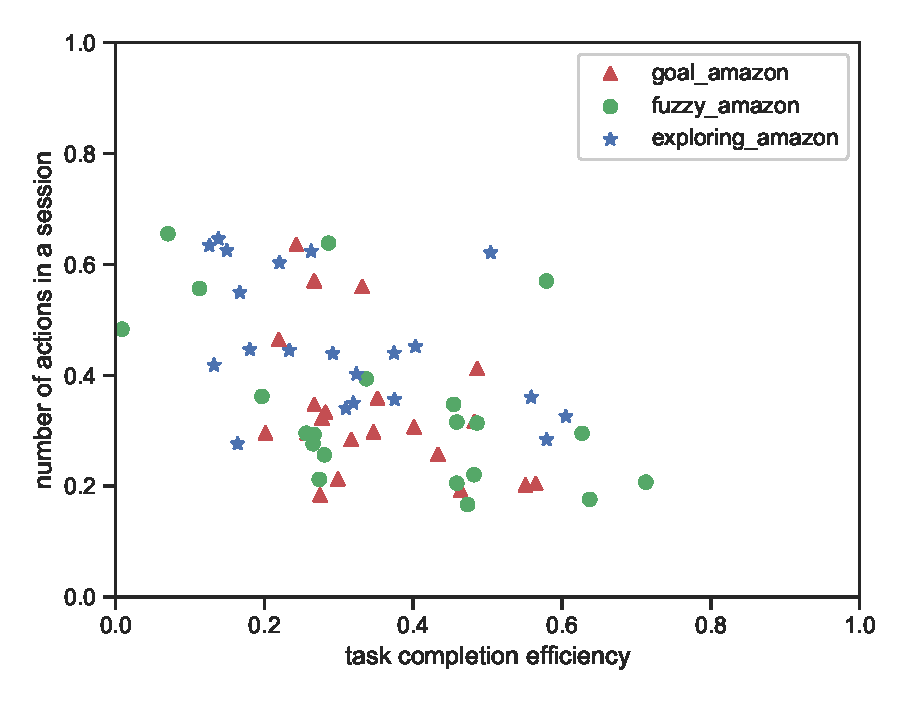
\includegraphics[width=0.25\textwidth]{figures/2d-eff-len-amazon}
    \includegraphics[width=0.25\textwidth]{figures/2d-len-dur-amazon}
    \caption{TODO:}
    \label{fig:general-amazon}
\end{figure}

TODO: table of classification report

more U-test, feature importance.

\subsubsection{Intepretation based on Action Path}
\label{sec:inter-action-path}

To use full capacity of our data, this section uses the entire clickstream and its corresponding
page-level stay time duration as input, three ending mark (<EOA\_GOAL>, <EOA\_FUZZY>, and <EOA\_EXPLORE>) 
as classification outputs, and then implements a single GRU layer action path model 
to classify the three type of tasks.

Our training parameters are: 
The GRU latent dimension is 10, training process feeds 151 clickstreams and 
propagates 500 epochs with batch size of 32.
In the end of training, we use Adam optimizer, evaluate on 38 clickstreams and 
archieved 100\% accuracy on our validation set.

The validation loss during the training is as shown in Figure \ref{fig:class-loss}.

\begin{figure}[H]
    \centering
    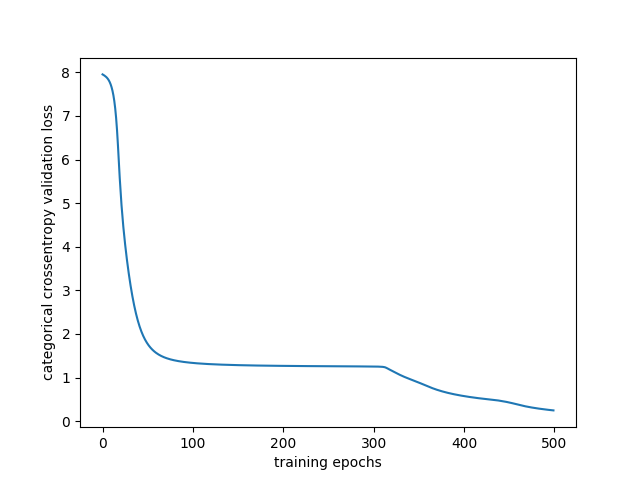
\includegraphics[width=0.75\textwidth]{figures/class-loss}
    \caption{Categorical Cross-Entropy Validation loss curve while 500 epoches. 
    The curves indicates the training process is not an overfitting since the loss is not increasing.}
    \label{fig:class-loss}
\end{figure}

One can observed that the training process is not an overfit, and the validation loss is 
still not increase after 500 epoches, thus, single GRU layer action path model 
remains a large expressive performance (100\% of three class classification in this dataset) 
when we have more data.

In addition, the action path model feeds the entire clickstream and time duration as inputs, 
therfore the entire clickstream contains informations regarding the number of visit actions
as well as completion effeciency and etc. Consequently, we conclude that the model works
perfectly on the classification of three different browsing behavior. Since our experiment is
only designed for three type of behavior, and the learning curve
shows the model still has capacity to classify more precise categories of browsing behavior,
perform a future investigation may be significance.

\subsection{Optimal Action Path Context}

This section we evaluates our model with limited action path context, where the feeding action path
are limited based on a split ratio. For instance, if a split ratio is 0.8 then we feed 80\% of 
an action path into the model, then predict the rest of 20\% actions. Figure \ref{} illustrates
the best accuracy we archieved for when use different split ratio.

\begin{figure}[H]
    \centering
    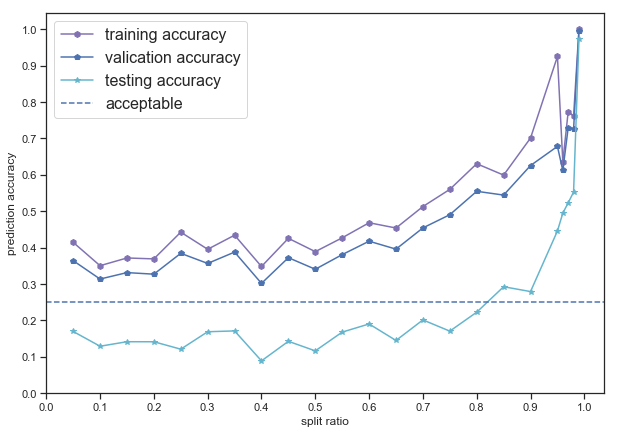
\includegraphics[width=0.7\textwidth]{figures/acc}
    \caption{TODO:}
    \label{fig:acc}
\end{figure}

\begin{figure}[H]
    \centering
    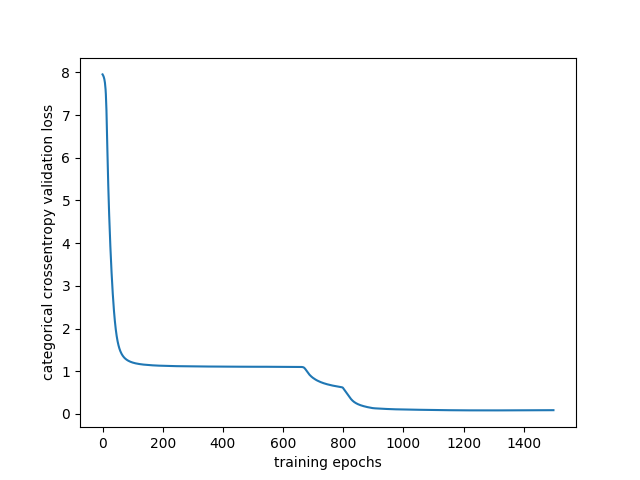
\includegraphics[width=0.45\textwidth]{figures/loss1}
    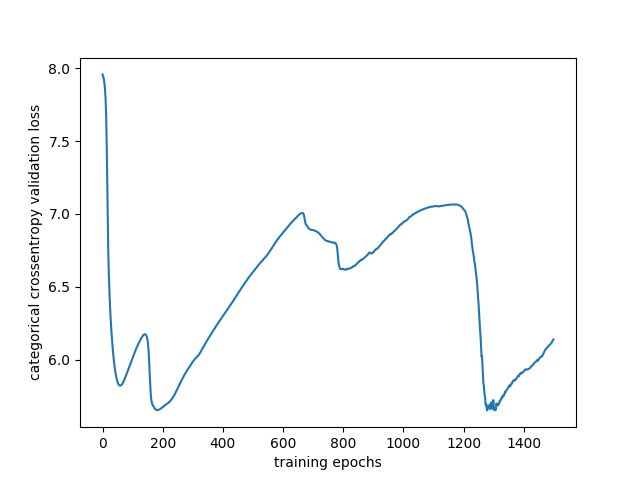
\includegraphics[width=0.45\textwidth]{figures/loss2}
    \caption{TODO:}
    \label{fig:loss}
\end{figure}


\subsection{Action Path Visualization}

This section visualizes the actual action path of users and discusses the behavior qualitatively.
Note that we collected 189 clickstream in total, which is not possible to illustrate all of them
in the thesis, we selected three typical clickstreams to discuss and provided a visualization tool
to help readers to explore them.

\subsubsection{Individual Common Patterns}

\begin{figure}[H]
    \centering
    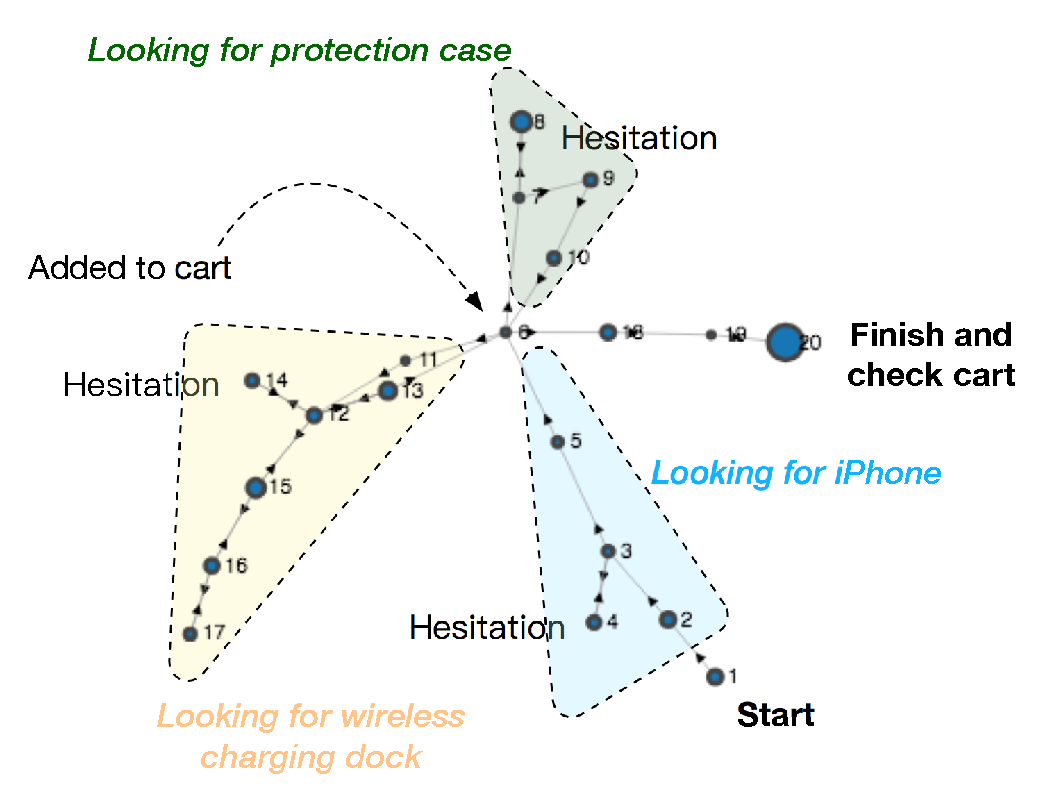
\includegraphics[width=0.45\textwidth]{figures/vis-goal1}
    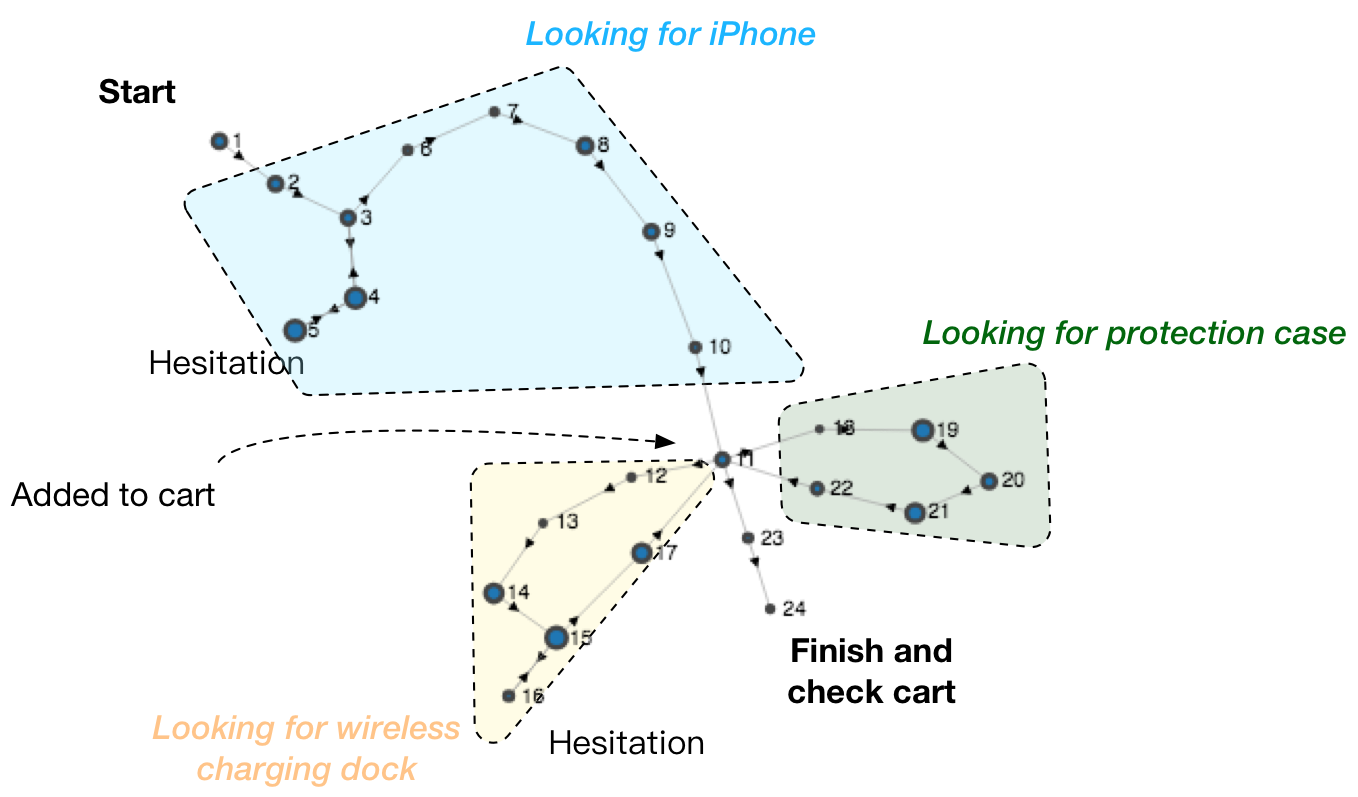
\includegraphics[width=0.45\textwidth]{figures/vis-goal2}
    \caption{TODO:}
    \label{fig:vis-goal}
\end{figure}


\begin{figure}[H]
    \centering
    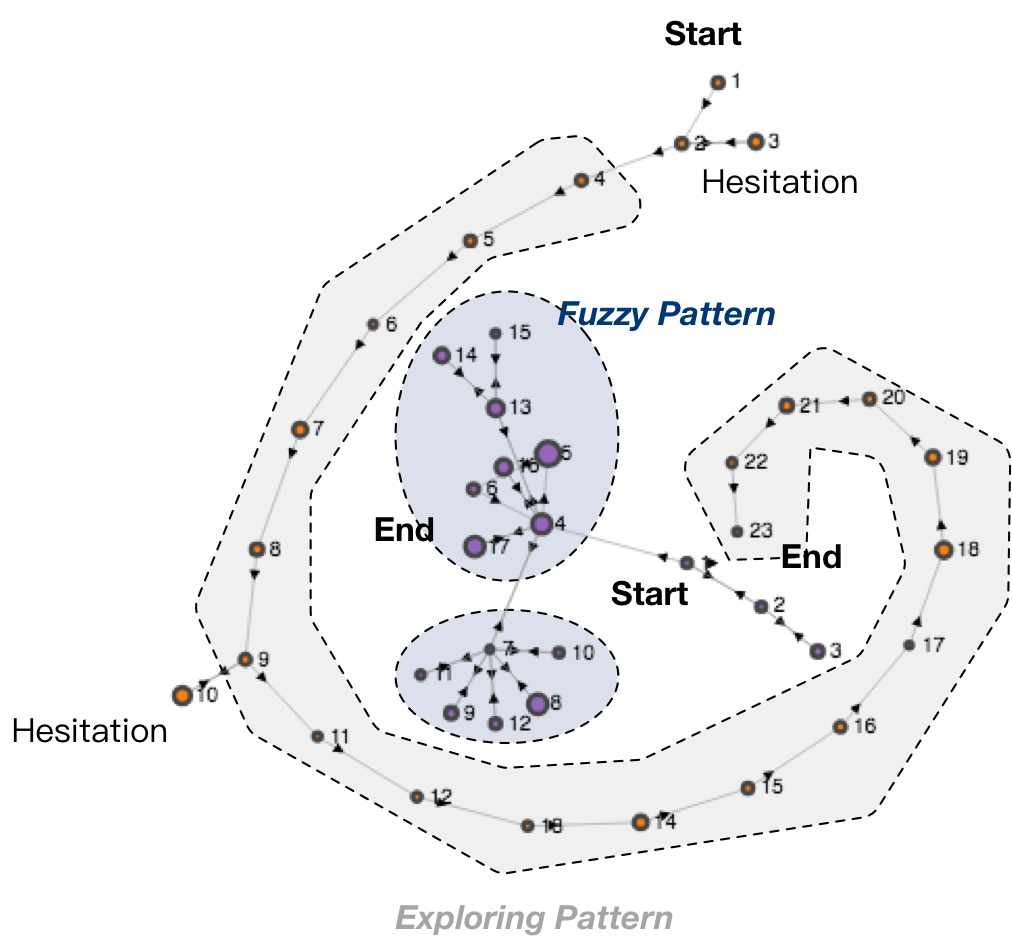
\includegraphics[width=0.45\textwidth]{figures/vis-fuzzy-explore1}
    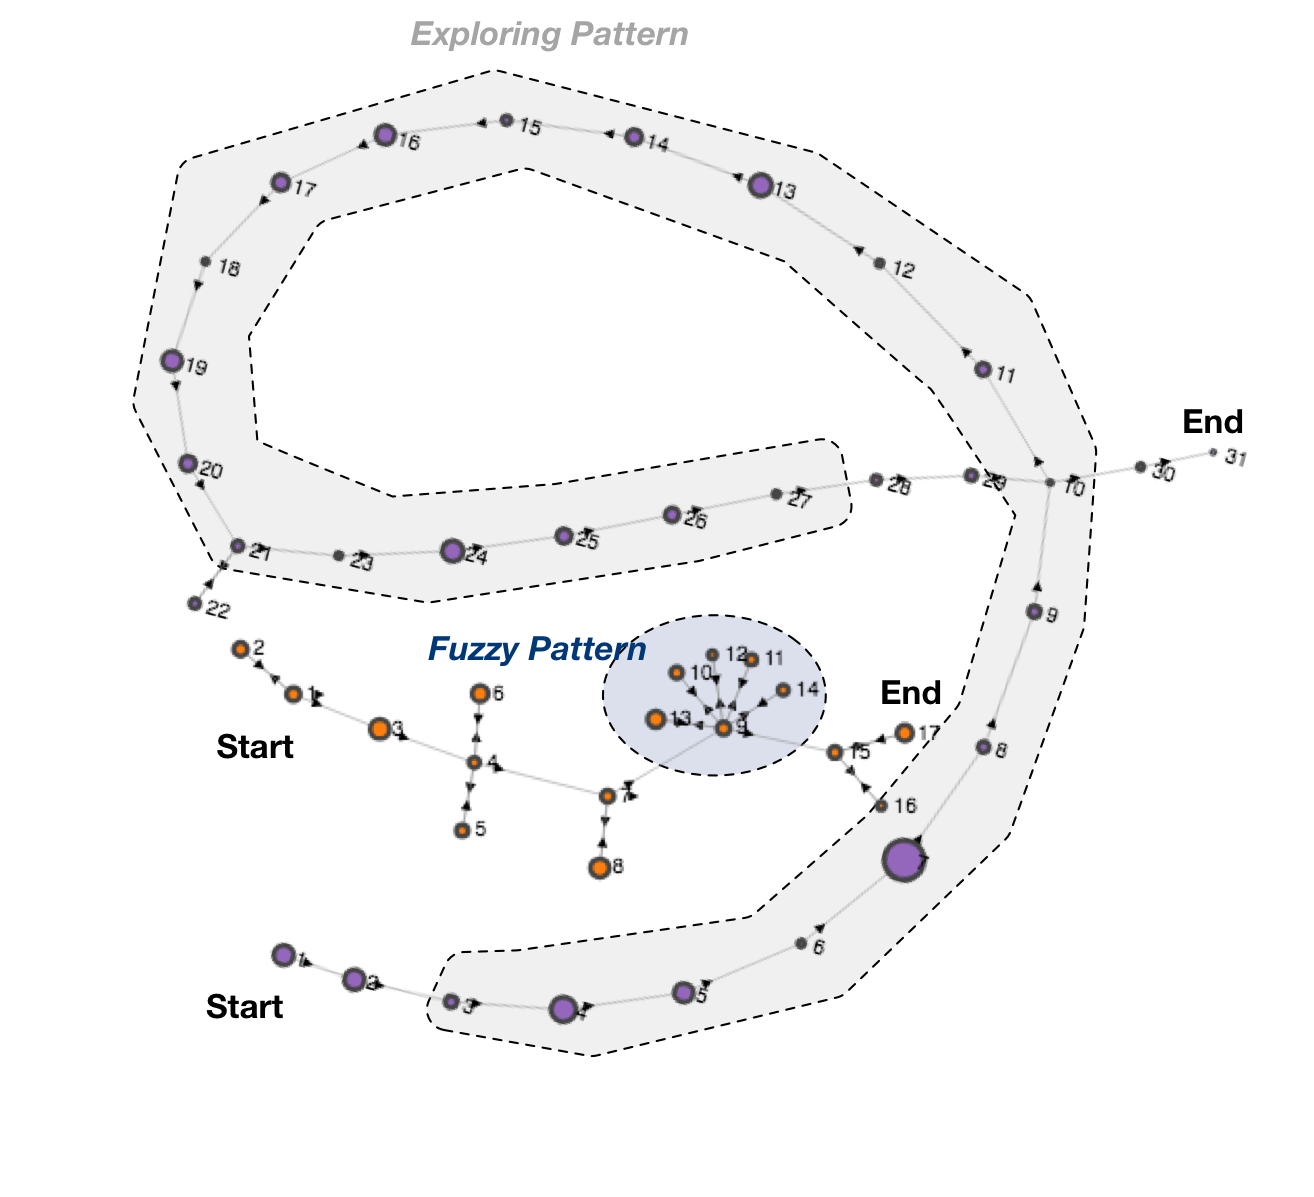
\includegraphics[width=0.45\textwidth]{figures/vis-fuzzy-explore2}
    \caption{TODO:}
    \label{fig:vis-fuzzy-explore}
\end{figure}

\subsubsection{Cross-user Overlap Patterns}

\begin{figure}[H]
    \centering
    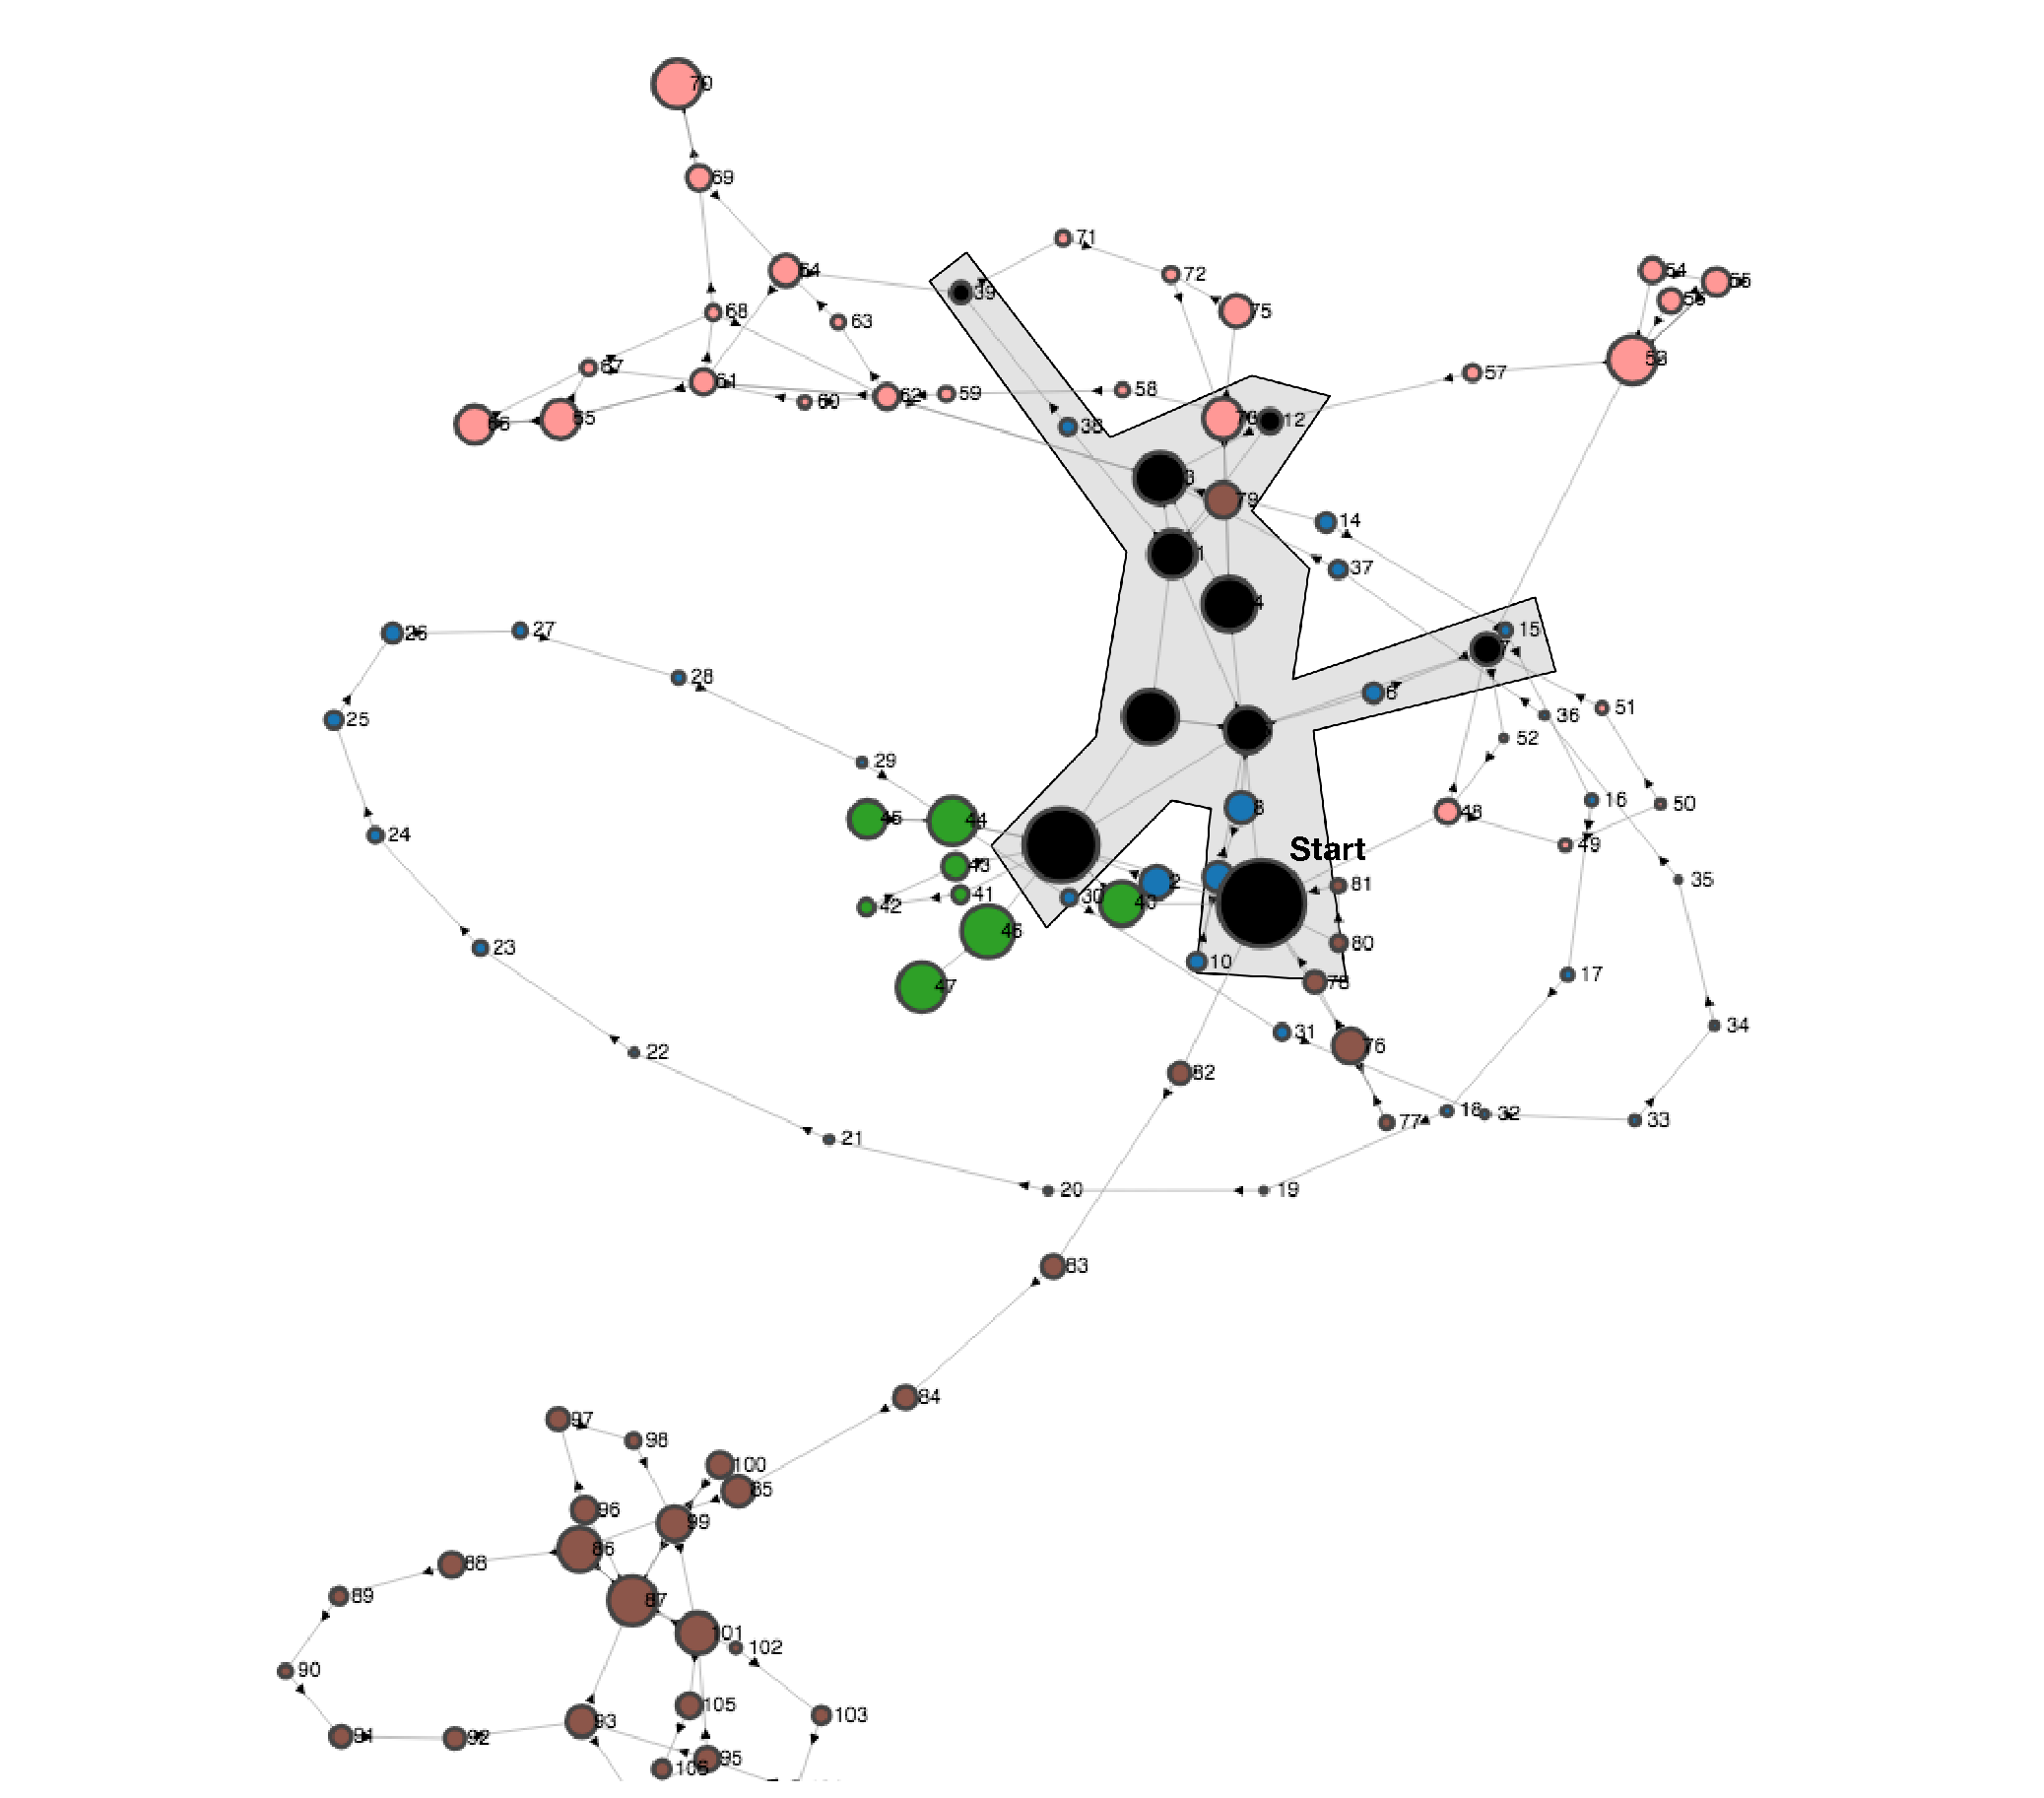
\includegraphics[width=0.45\textwidth]{figures/overlap1}
    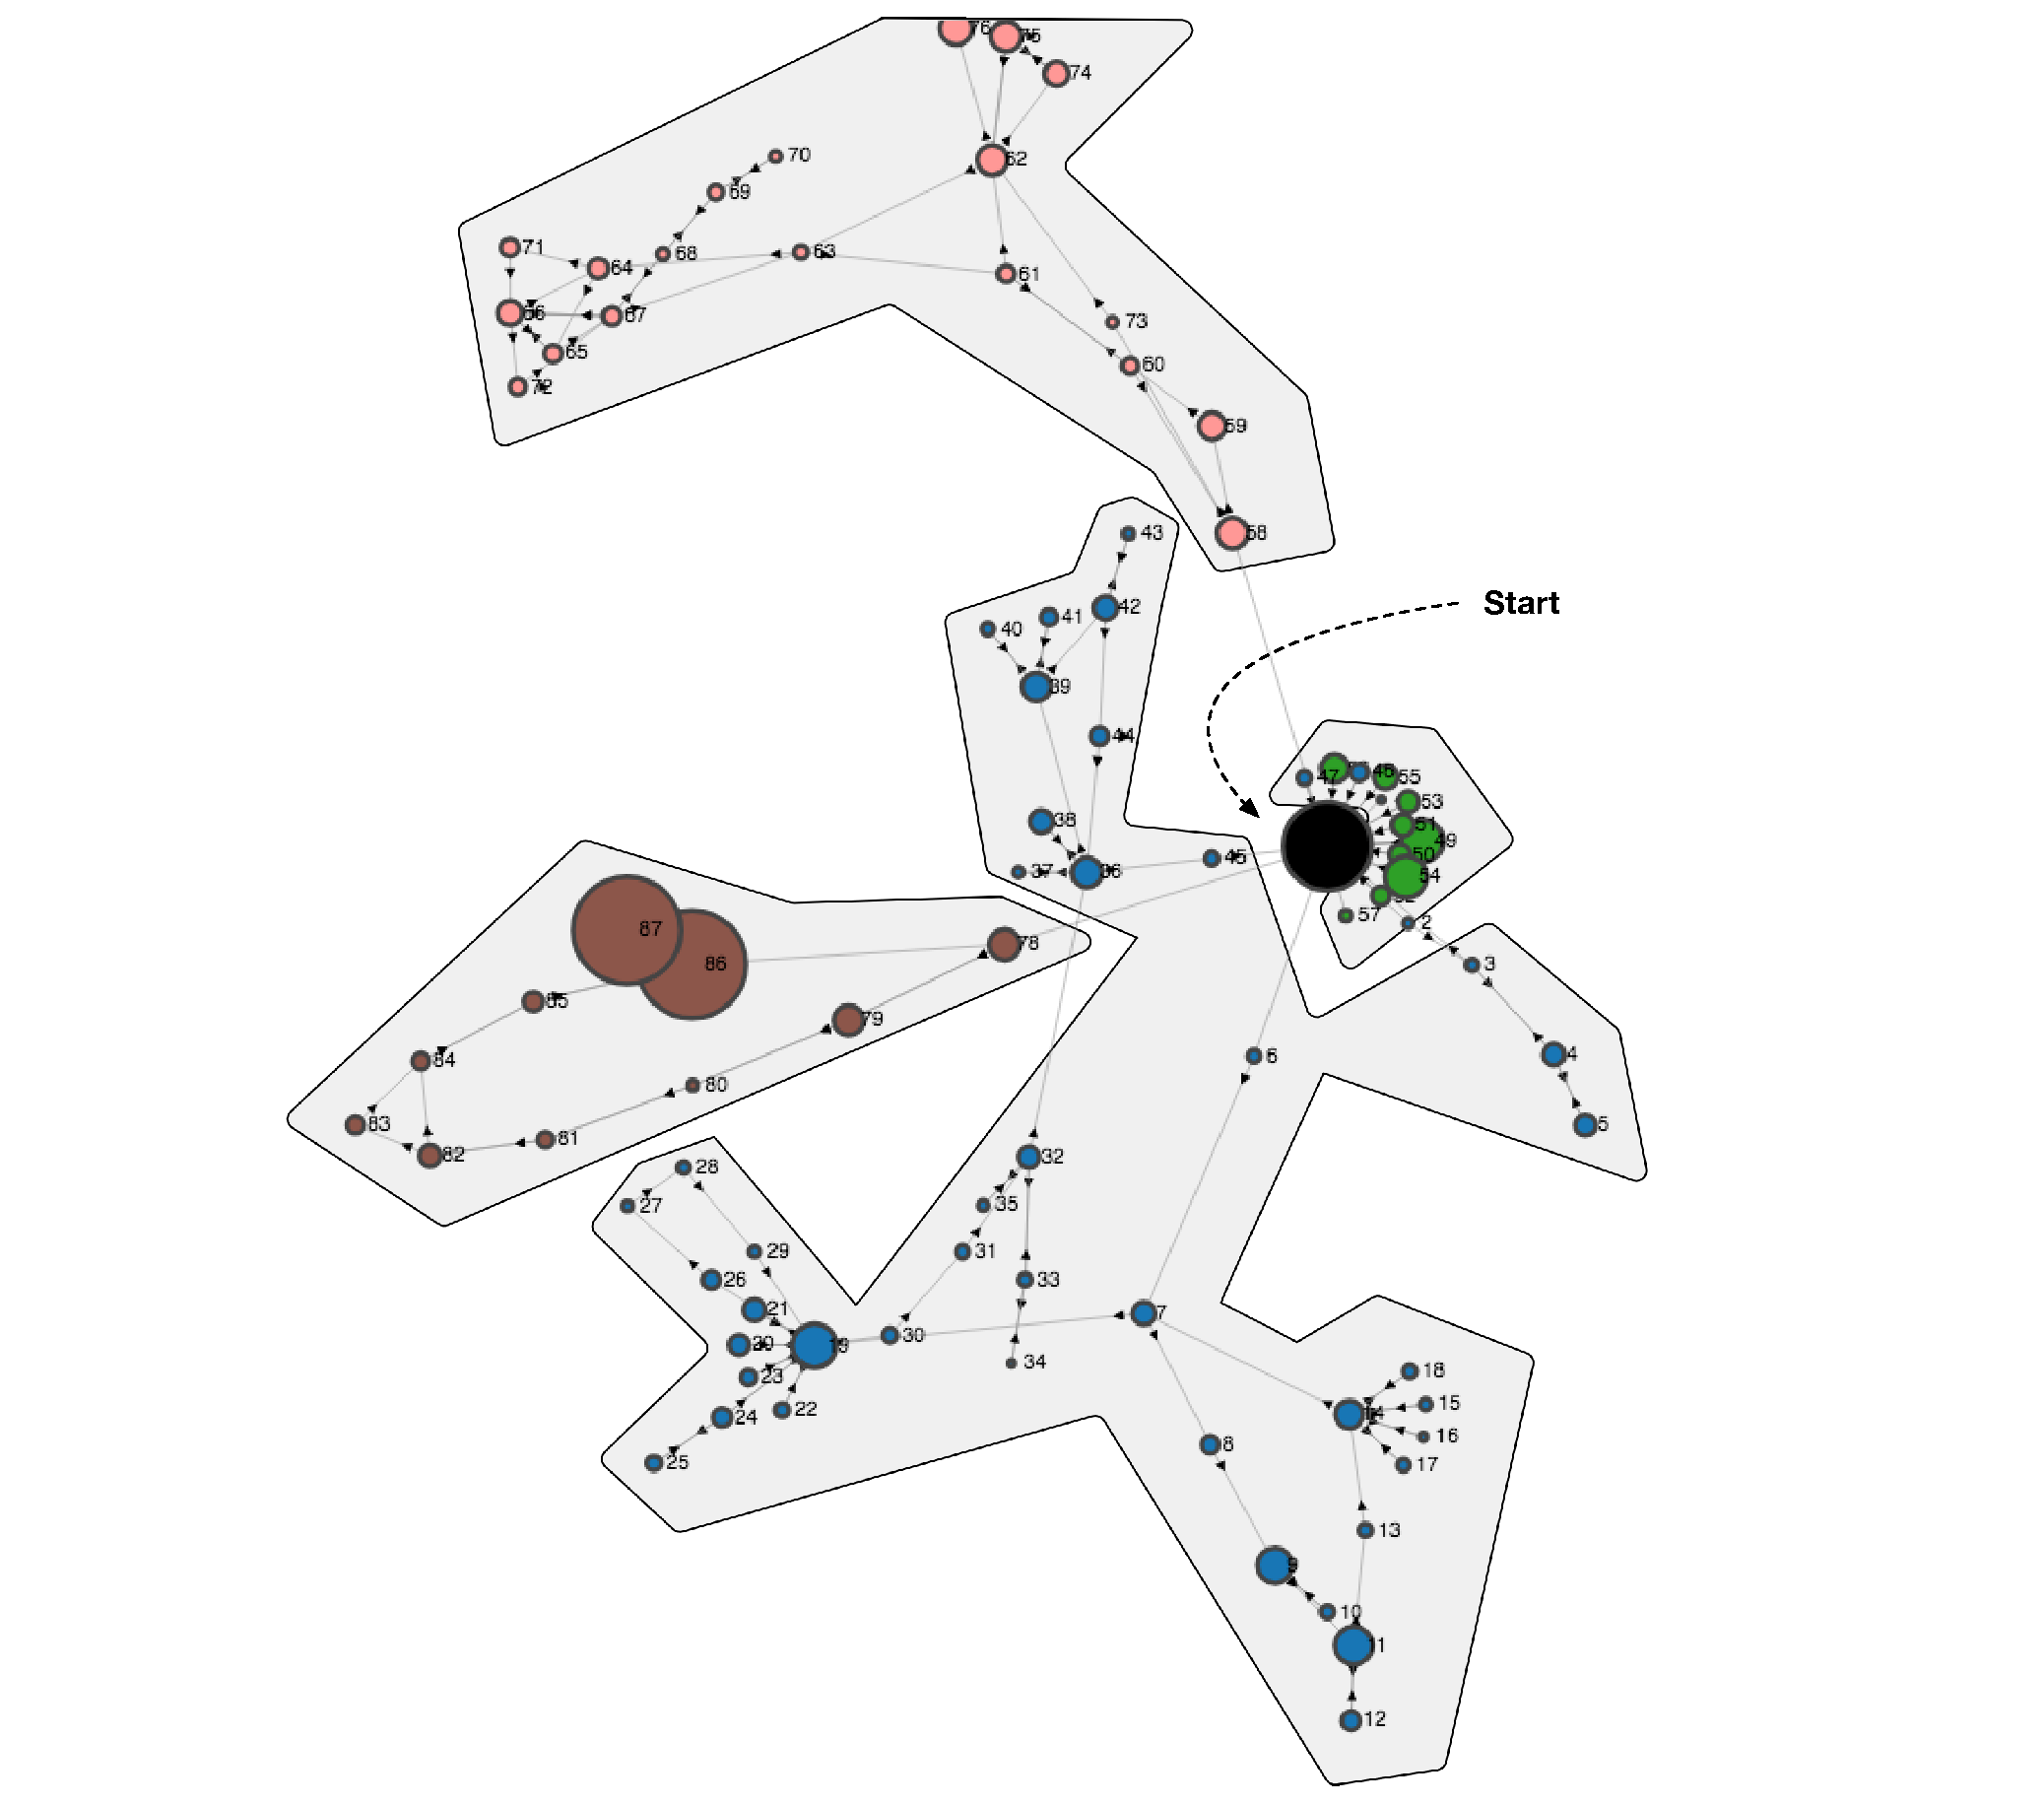
\includegraphics[width=0.45\textwidth]{figures/overlap2}
    \caption{TODO:}
    \label{fig:overlap}
\end{figure}



\cleardoublepage
\section{Applications}
\label{ch:app}

\epigraph{Simplicity is Complicated.}{Rob Pike}

This chapter we first introduce a possible application of our proposed model
including the implemented feature, how it could benefit a user, as well as the 
architecture and dataflow within the application.
Then in the second part of this chapter, we formalize and discusse 
the possibility and benefits as a standard Web API to web developers and website designer.

\subsection{Client-side Browser Plugin}
\label{sec:plugin}

We developed a client-side browser plugin is an illustration of our model applications.
The plugin is an intelligent system that proactively serves its user, 
and it provides proactive notification based on the historical actions in a session
when browsing behavior is detected as goal-oriented or fuzzy behavior, 
as illustrated in Figure \ref{fig:proactive-noti}.

\begin{figure}[H]
    \centering
    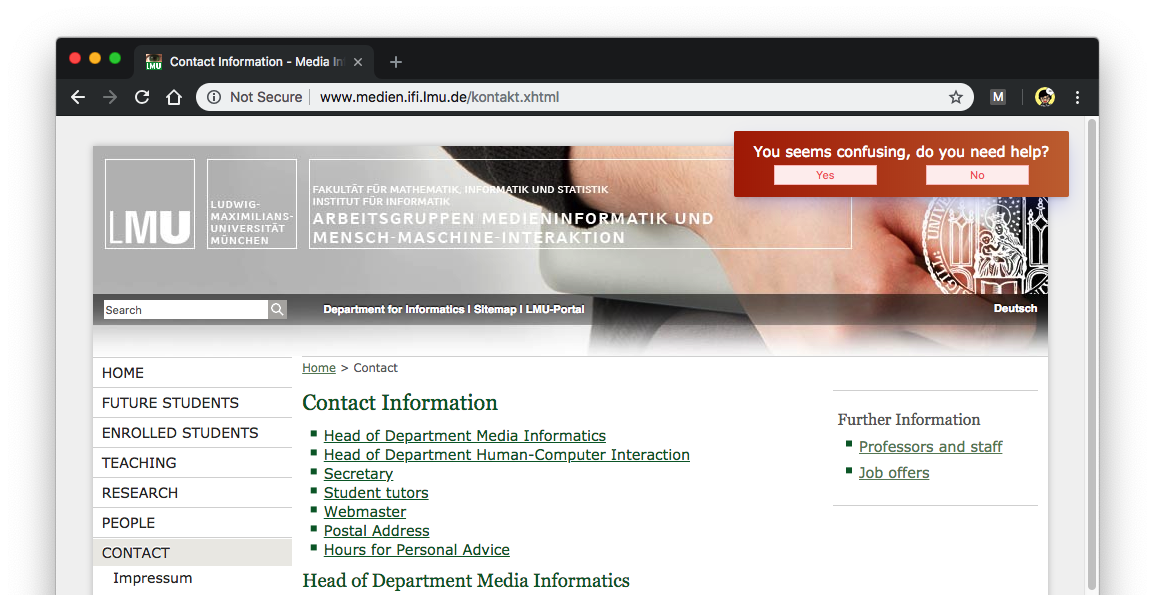
\includegraphics[width=0.7\textwidth]{figures/proactive-noti}
    \caption{Proactive notification:
    The plugin injects monitor script when the page is loaded, and then serve user giving
    notification when detecting fuzzy browsing behavior.}
    \label{fig:proactive-noti}
\end{figure}

The user can either select ``Yes'' and navigates to the most likely page that he/she will visit
in the future, or select ``No'' to ignore the notification.
The plugin serves user only if the browsing behavior is detected as fuzzy behavior because
of the forbear of notification. We argue that the plugin is only a supplementary of improving
browsing experience but not always necessary, for instance in exploring behavior, information
need of a user may not be clearly observed and the recommendations are not usefulness. 
One of the benefits of the plugin is to proactively help the user become efficient
and reach the destination as fast as possible in goal-oriented browsing.

\begin{figure}[H]
    \centering
    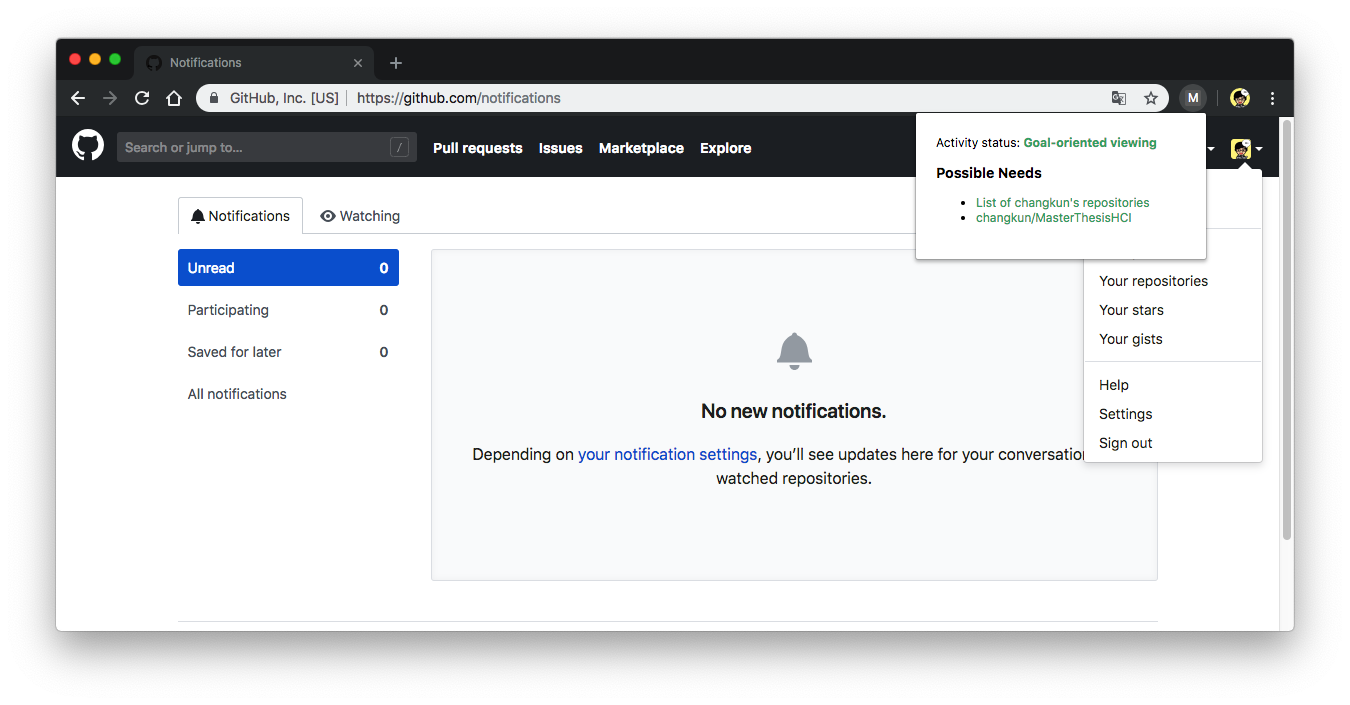
\includegraphics[width=0.7\textwidth]{figures/plugin-predicting-result}
    \caption{The plugin provided popup page: users can always open the page
    to understand the current status of browsing and predicted needs based on
    historical actions in a browsing session. In this case, the detected browsing behavior
    is under goal-oriented browsing, and predicted actions
    are accessing the page of public repositories and accessing a specific repository.}
    \label{fig:plugin-predict}
\end{figure}

In Figure \ref{fig:plugin-predict}, except proactive notification, 
users can always open a popup page provided by the plugin.
The popup page provides another interaction that gives the predicted needs 
based on historical user actions. A user can always interact with the plugin and
retrieve the possible needs and browsing status in the current session.
These information are helpful to the plugin user because the user can understand
what is the current status of web browsing, which implicitly aware the person better focus
if the person detected as exploring browsing behavior.

\begin{figure}[H]
    \centering
    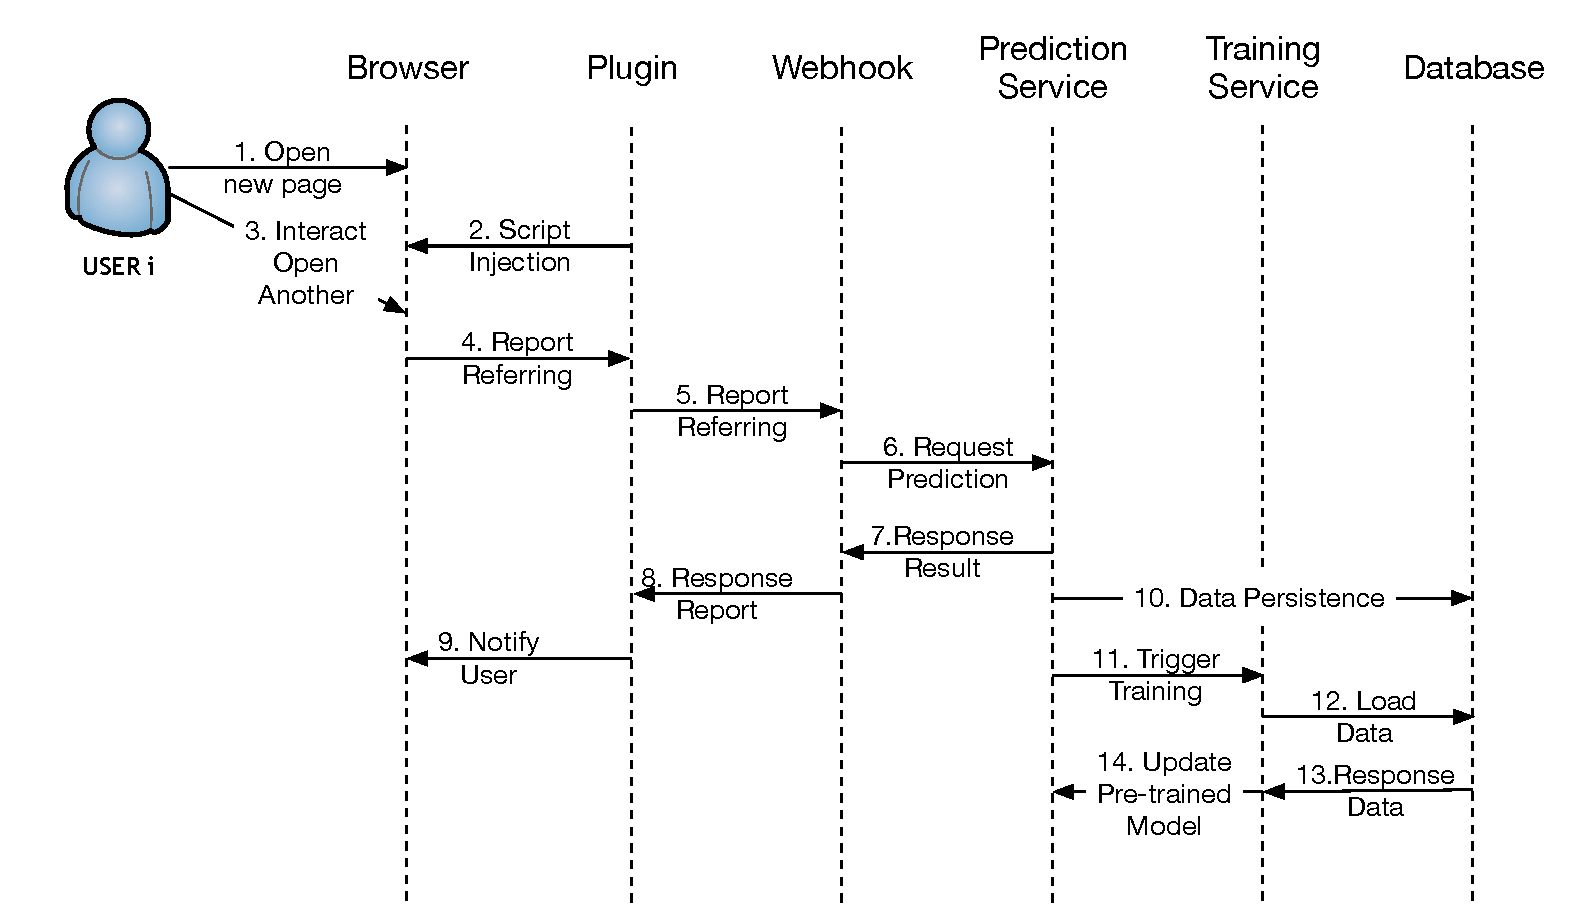
\includegraphics[width=0.7\textwidth]{figures/arch}
    \caption{The implemented architecture of our plugin}
    \label{fig:arch}
\end{figure}

The implementation and architecture is not simple
despite it provides a small feature that exhibit context and future inforamtion to the user.
Figure \ref{fig:arch} illustrates the implemented architecture of the plugin.

First of all, the plugin daemon process will inject monitoring script (\emph{step2}) to 
the newly opened page (\emph{step1}).
When user start browsing and interacting (\emph{step3}), the injected script will report the referring of
previous visited URL, current URL and stay duration to the daemon process of the plugin (\emph{step4}).

Afterwards, the daemon process will report the referring information to the plguin server webhook (\emph{step5}),
and then the webhook will immediatelly request the intra prediction microservice (\emph{step6}) and resulting a 
prediction (\emph{step7}) then response a prediction result to the daemon process 
by using a pre-trained model (\emph{step8}). Therefore the daemon process can decide 
if a proactive notification should be presented to the user or simply update its popup page
just for illustration (\emph{step9}).

Since the prediction service received a new user action, it stores the action into database
subsequently for model update (\emph{step10}). Because of the cost of train a new model,
the prediction service can decide to trigger training service to retrain the model 
if already received enough new data (\emph{step11}). 
Further, the training service uses the pre-trained model as
a base model to initiate the training by request newly created data from databse (\emph{step12} and \emph{step13}), 
similar to the idea of transfer learning.
After the training achieved a compatible performance comparing to the pre-trained model,
the training service will update the newly trained model to the prediction service (\emph{step14}), which 
serves future prediciton requests.

As we can observe from the architecture, the infrastructure is not as simple as the plugin feature
intent to provide, therefore we argue that it is a feature that only browser manufactures
can provide. In the following section, we formalize and discuss 
the possibilities of the plugin feature as a Web API.

\subsection{Web API Standardization and Platform-as-a-Service}

Web APIs is a generic term used in various fields of development.
Web APIs in a context of web browsers mainly indicates the APIs provided
by browser manufactures to developers that helps web application can even close
to manipulate hardwares, for instance, WebAssembly \cite{w3c2018ws}.

Nowadays, there are experimental standard Web APIs integrates complex features to 
web developers, e.g. Web Speech APIs \cite{mozilla2019speech}, and 
only Google Chrome (after version 24) support. 
The specification proposal was initiated by Google, according to 
the source code of Chromium Kernel, the APIs are implemented based on 
the speech recognition service provided 
by Google Cloud Platform 
\footnote{\url{https://github.com/chromium/chromium/blob/83928864c18362a4b0f84bad9bee4104f4655430/content/browser/speech/speech\_recognition\_engine.cc\#L35}, last accessed on January 03, 2019},
which provides us a signal that browser APIs does not only giving interfaces to
the hardware, but also access cloud platform services, i.e. Platform-as-a-Service integrated 
APIs.

The plugin we illustrated in Section \ref{sec:plugin} can also be integrated as a PaaS API
that embedded into web browsers, which simplifies the infrastructure of the plugin. 
As a developer, one can simply call the standardized API to report current user actions
then get a response of current behavior status and the prediction of future movement or 
actions, as the diagram shown in Figure \ref{fig:webapi}.

\begin{figure}[H]
    \centering
    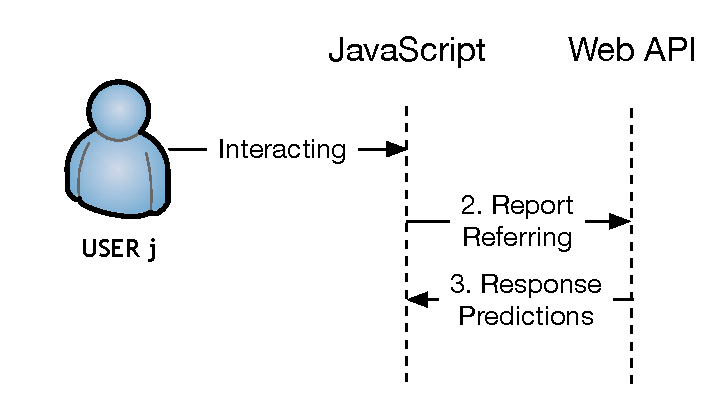
\includegraphics[width=0.4\textwidth]{figures/webapi}
    \caption{Usage overview of standadized BrowsingBehavior API}
    \label{fig:webapi}
\end{figure}

Defining the specification of the Paas API aims enable web developers to
monitoring, in a web browser, the future actions of their user.
Developers can use the predicted actions to dynamically change the UI elements then improve
the user experience of their product. To keep the API to a minimum, we breifly discuss the
non-normative web API design of the browsing behavior predictor.

\subsubsection{The \emph{BrowsingBehavior} Interface}

The browsing behavior interface is the scripted web API for resulting a monitored browsing
session, which is presented in Code \ref{lst:interface}.

\begin{lstlisting}[
    language={JavaScript},
    caption={BrowsingBehavior Interface},
    label={lst:interface}
]
[Exposed=Window, Constructor]
interface BrowsingBehavior : EventTarget {
    
    // methods to drive browsing behavior response
    void start();
    void stop();
    void pause();
    void resume();

    // event methods
    attribute EventHandler onBrowsingStart;
    attribute EventHandler onBrowsingEnd;
    attribute EventHandler onBrowsingPause;
    attribute EventHandler onBrowsingResume;
    attribute EventHandler onResult;
}
\end{lstlisting}

\paragraph{\emph{start()} method} When start method is called, it represents the moment in
time the web application wishes to begin monitoring user's actions.
Then every step when user making actions, the \emph{EventHandler onResult} will produce
a standard prediction and classification of user browsing behavior. Further, 
the \emph{EventHandler onBrowsingStart} will be called immediatelly after calling 
this method and before resulting a prediction result, which gives a barrier in between of
calling \emph{start} and callback \emph{onResult}.

\paragraph{\emph{stop()} method} When stop method is called, it represents the instruction
to browsing behavior service to stop monitoring user actions, and resulting a final 
prediction in the \emph{EventHandler onBrowsingEnd}.

\paragraph{\emph{pause()} method} This method is used to ignoring the upcoming user actions
to pauses the monitoring of user actions, and resulting a prediction in the 
\emph{EventHandler onBrowsingPause}.

\paragraph{\emph{resume()} method} This method resumes the paused \emph{BrowsingBehavior}
object and recover the monitoring of user actions. Before monitoring is fully recovered,
the \emph{EventHandler onBrowsingResume} will be called.

The major consideration of designing these four methods is to restrict an abuse of the APIs.
Similar to cookie, speech recognition APIs, a website should acquire an authorization from
their user, otherwise the API cannot monitor any user actions on the web, which partially
solves the issue of privacy and security. We will discuss more concerns of the feature in
Chapter \ref{ch:discuss}.

\subsubsection{\emph{onResult} callback}

\emph{onResult} callback passes the prediction after the browser user performed an action.
The prediction result consist two parts: behavior and future movements.

The \emph{behavior} attribute of the result object is a JSON object that contains 
confidence level, i.e. classification probability, and a enumerate \emph{category} attribute
that indicate the a finite set of user browsing behaviors, i.e. goal-oriented, fuzzy or exploring.

\begin{lstlisting}[
    language={JavaScript},
    caption={Result object of onResult callback},
    label={lst:callback}
]
{
    "behavior": {
        "confidence": float64,
        "category": string,
    },
    "futures": [
        {
            "confidence": float64,
            "actions": array[string],
        },
        {
            "confidence": float64,
            "actions": array[string],
        },
        ...
    ]
}
\end{lstlisting}

The \emph{futures} attribute of the result object is an ordered JSON object that from the
highest \emph{confidence} to lowerest {confidence} and the \emph{confidence} is a floating
number from minimum 0 to maximum 1 value. Meanwhile, the \emph{actions} attribute in a 
JSON object of an item of \emph{futures} array is an array of possible actions of URLs that
ordered in chronologic order, the first element represents the next immediate action,
and the last element represents the final action in the session, as shown in Code \ref{lst:callback}.

\begin{lstlisting}[
    language={JavaScript},
    caption={Formation of browser collections},
    label={lst:collect}
]
{
    "device_id": string,
    "previous_url": string,
    "current_url": string,
    "stay_seconds": float64,
    "time": string
}
\end{lstlisting}

From the perspective of implementation, browser manufactures collect data after developer
calls \emph{start()}.
In Code \ref{lst:collect}, each time when user performs an action, including open a new page,
switch to another tab or backtrack to former page, will result an JSON object that contains
\emph{device\_id} a unique identifier that represents the device, \emph{previous\_url} the previous
URL of the action, \emph{current\_url} the current URL of the action, \emph{stay\_seconds}
the stay duration of \emph{previous\_url} and \emph{time} string of the time of data creation.

% \subsubsection{Communication Protocol}

\cleardoublepage
\section{Discussion}

% \subsection{Discussion}

% \subsection{Future Work}

% 1. limitations

% 2. what could improve

% 3. whats next


% 讨论 google 的一步 prefetching

% 讨论这些数据在移动端的使用

% 讨论这些模式对用户的帮助
\section{Conclusions}
\label{ch:final}

\subsection{Summary}

% 1. what has been done

This thesis proposed an action path model that describes client-side user clickstream.
To justify our model, we designed nine browsing tasks for three qualitatively
discussed browsing behavior based on the theory of information behavior, then 
held a user study for these tasks that simulates the behaviors. 
Afterwards, we applied the collected data from user study to our action path model and
analysed the model performance to these data with comparison to traditional machine 
learning approach.
Subsequently, we also visualized these data and closely discovered the common, 
individual and intersection patterns among client-side clickstream.
As an application show case, we illustrated a browser plugin that monitors client-side 
user clickstream to predict future movements of web browsing and discussed the benifits of this plugin.
Futhermore, we presented a generic architecture communication flow and architecture of the plugin, 
as well as the possibilities of standardize the plugin feature as browser Web APIs to other developers.

% 2. what are the findings

Our finding indicates the completion difficulty in different type of tasks are significant different,
especially the difficulty of fuzzy task is significant difficult than goal-oriented task,
and the goal-oriented task is also significant difficult than exploring task.
For completion efficiency, length of client-side clickstream and total duration of the clickstream

% 3. emphasize the importance >> place to large context
Our findings are generic and subservience. The model can not only be use on desktop but
also can be implemented in a mobilephone, or even a outside the context of web browsing. 
Similar to other user behavior data, client-side user clickstream or user actions 
directly indicates movements of a user and how they making decisions. Understanding, 
interpreting and predicting these data not only improves the user experience when doing
web browsing, but also useful to help users reducing useless browsing, better controls 
and manages their time. Moreover, by standardize the data processing process can formalize
the feature to developers, and then help them using the behavior predictions to
improve their product user experience.

% 4. summarize / conclude
Traditional server collected clickstream data has been proved its high value in many fields. With our work we exposit the value one-step forward, and contributes to models and approaches that hope to bring ponderable research to the community.


\cleardoublepage
\part*{Appendix}
\appendix
\addcontentsline{toc}{part}{Appendix}
% No headline on top of each page
\fancyhead[LE,RO,LO,RE]{}

All resources relates to the thesis are open source, they can be found publicly in:

\begin{itemize}
    \item Thesis homepage: \url{https://changkun.us/master-thesis-hci/};
    \item GitHub repostory: \url{https://github.com/changkun/MasterThesisHCI/}.
\end{itemize}

All related text, picture and video content are licensed under a Creative Commons Attribution-NonCommercial-ShareAlike 4.0 International License\footnote{\url{http://creativecommons.org/licenses/by-nc-sa/4.0/}}.
The other parts of the thesis (such as program source code) are licensed under a MIT Public License\footnote{\url{https://github.com/changkun/MasterThesisHCI/blob/master/LICENSE}}.

\section{Content of enclosed USB}
\label{appendix:a}

\begin{enumerate}
    \item $/documents/$ - TODO
\end{enumerate}

\part*{Bibliography}

\addcontentsline{toc}{part}{Bibliography}
\nocite{*}
\bibliographystyle{plain}
\bibliography{literature/list}
\end{document}